% !TEX root = ../sethomas_thesis_main.tex

\section{Kirigami inspired Compliant SMA Actuators}
Using topology optimization, various compliant SMA actuators can be designed with the intent to combine the functions of the kinematic stage and the active element. However, due to the current limitations of fabrication and its costs, the feasibility of such an actuator, in the current sense, is unlikely. As additive manufacturing of SMAs becomes more accessible, the advantages of designing compliant SMA structures such as increasing the overall work density of the actuator, will become more apparent and attractive.

Kirigami, the Japanese art of cutting paper to create intricate structure, has gained traction in various engineering fields to create stretchable structure as shown in the work by \cite{tangProgrammableKiriKirigamiMetamaterials2017}. While designing 3D compliant structure made of SMA is expensive, this kirigami approach can be extended to SMAs to create compliant structures that when cut in a specific manner, can exhibit surprising mechanical behaviours.

When designing actuators, a key detail to keep in mind is the life cycle of the device. In common industrial applications, the number of cycles to fatigue of traditional grippers can exceed $10^6$ cycles. In the case of SMA actuators, this number is much lower and is directly related to the structural fatigue of the material. The determining factors regarding the fatigue life of SMAs are the strain amplitude and the type of strain applied to the material. The work by \cite{runcimanEquivalentStrainCoffin2011} looks at the fatigue lifetime of NiTiNOL based on different loading conditions, such as torsion, tension and bending. They conclude that SMAs tend to have a much longer life cycle when loading under torsion or bending when compared to tension. The results show that with a fixed strain amplitude of 1\%, in tension, the number of cycles to failure is less than $10^3$ whereas in bending or torsion, the number of cycles to failure is around $10^5$.

The availability of NiTiNOL in different geometries such as springs, wires and sheets, has allowed the creation of multiple classes of SMA actuators that exploit their respective advantages. As mentioned in previous sections, the simplest approach would be to use the alloy in the shape of a wire paired with a biasing spring to drive an actuator where the stress and strain of the material corresponds directly to the stroke and force output of the actuator. In these cases, SMA wires are elongated under pure traction and are then heated to recover the strain and provide the force output as shown in the works by \cite{kyungDesignMicrogripperMicromanipulation2008}, \cite{welschVacuumGripperSystem2018}, \cite{haibinModelingGraspingForce2018}, and \cite{andrianesisDevelopmentControlMultifunctional2015}. Here, the stroke of the actuator can not exceed 1\% without compromising its fatigue life. Thus, in cases where a larger stroke is required, the geometry of the wire is adapted to form a spring which can provide stroke above 100\% as implemented in the works by \cite{ikutaMicroMiniatureShape1990} and \cite{zhakypovOrigamiInspiredReconfigurableSuction2018}. Here, the material no longer deforms in traction but rather in torsion, thereby increasing its fatigue life but while compromising the force output. This implies that there is a trade-off to be made between the force output, and the stroke and fatigue life.

Since SMAs are available in the form of sheets which can be machined using laser cutters into complex geometries, different kinds of SMA actuator systems exploit the longer fatigue life of SMAs in flexion to create novel grippers as shown in the works by \cite{kohlSMAMicrogripperSystem2002}, \cite{benardThinfilmShapememoryAlloy1998}, \cite{zhakypovOrigamiInspiredReconfigurableSuction2018}. The major advantage to using sheets instead of wires is the fact that they provide a much higher force output. The difference in force output between sheets and wires can be reduced by placing multiple wires in parallel to generate forces in the same order of magnitude as sheets. Thus in applications, where a higher force output is required, the use of SMA sheets or multiple wires in parallel can be a viable solution.

When working with thin wires, placing them in parallel to augment the overall force output also increases the complexity of the system greatly. The manufacturing and assembly of such a system can be difficult. Furthermore, it is also impossible to uniformly deform all the wires equally, resulting in some wires being inactive during the shape memory effect. Thus, in cases where a higher force output is required, the design space can become limited to just using sheets. For maximum force output, the sheet can be elongated in pure traction but only up to about 1\%. In applications where a large stroke and force output is required, the SMA sheets in its original state is no longer viable. Traditionally, this limitation is overcome by adding a kinematic stage to amplify the stroke of the SMA actuator but comes with the cost of reduced overall work density of the final actuator.

In this section, a novel approach will look at a new kirigami-based approach to designing SMA sheets to obtain an actuator that can provide higher force output while being able to also provide high strokes. Kirigami is a variation of origami that involves the cutting of the substrate to create different shapes and behaviours. The pattern presented in this paper is based on the work by \cite{shyuKirigamiApproachEngineering2015} where a nanocomposite substrate is patterned to create a stretchable element. This approach allows an SMA sheet to reach strains over 100\% without losing its capacity to deliver a high force output.

\subsection{Proposed Patterns}
The pattern plays the most important role when creating a kirigami-inspired SMA actuator. The pattern when cut into the SMA sheet creates a meta-material that alters the mechanical properties from the original material. Based on the pattern used, various different behaviours such as stroke amplification or movement conversion can be imparted into the sheet. In this work, as seen in \cref{fig:sma-kiri-patterns}, two patterns are explored. The $\Omega$-pattern, taken from the work by \cite{shyuKirigamiApproachEngineering2015}, provides an amplification of the stroke while also deforming the SMA in flexion which is favourable for the overall fatigue of the material. The second pattern consists of the Lotus-pattern which allows the material to rotate around its centre. Furthermore, if fabricated using SMA and actuated, this pattern can be used to an active smart pivot.

% insert undeformed (maybe deformed also) picture of the patterns
\begin{figure}[hbt]
     \centering
     \begin{subfigure}[b]{0.45\textwidth}
         \centering
         \includegraphics[height=0.66\textwidth,angle=180]{images/chap5/sma-kiri-unit-grey.png}
         \caption{$\Omega$-pattern}
         \label{fig:omega-pattern-simple}
     \end{subfigure}
     % \hfill
     \begin{subfigure}[b]{0.45\textwidth}
         \centering
         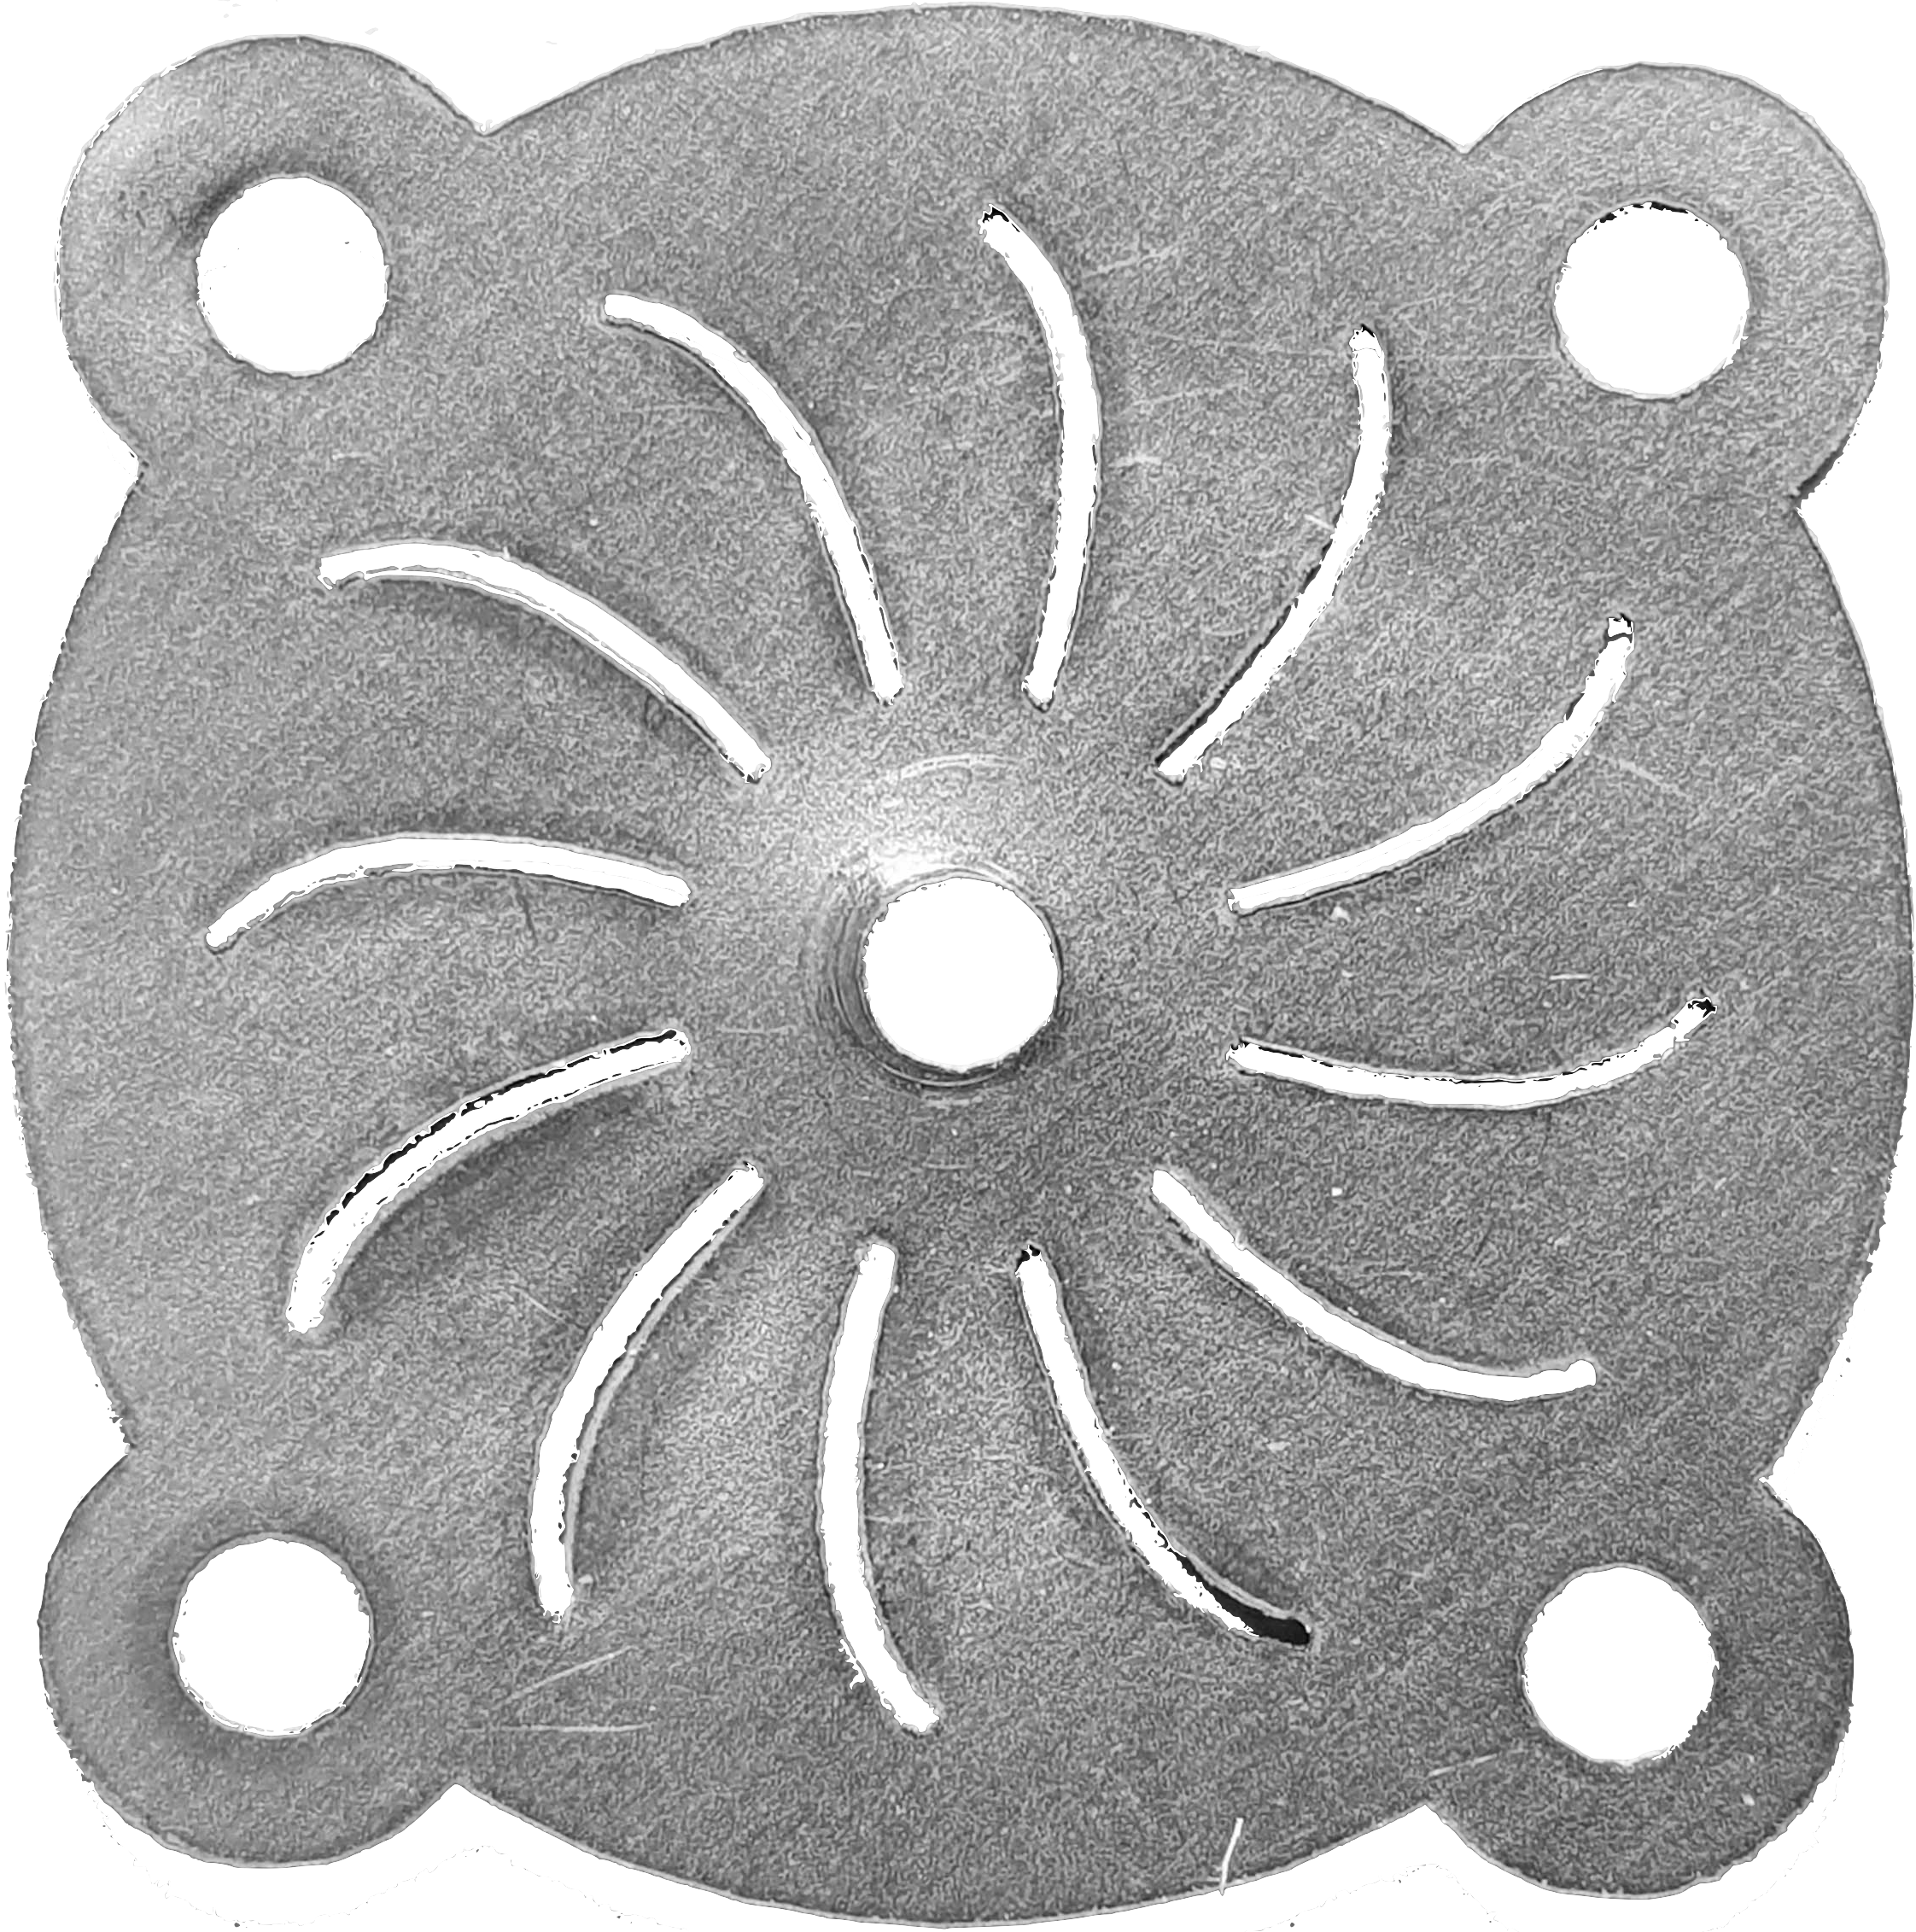
\includegraphics[height=0.66\textwidth]{images/chap5/sma-kiri-lotus-fixation-grey.png}
         \caption{Lotus-pattern}
         \label{fig:lotus-pattern-simple}
     \end{subfigure}
    \caption{The proposed kirigami patterns for the SMA actuator where (a) allows for a large stroke linear elongation while (b) allows a rotation around its centre.}
    \label{fig:sma-kiri-patterns}
\end{figure}

These patterned structures make use of out-of-plane deformation to create the desired mechanical properties such as stroke amplification. These highly stretchable sheets, when exposed to an imposed force or moment, make use of the out-of-plane deformation of each individual pattern to elongate beyond the capabilities of the material on its own. Due to the fact that these deformations are irregular and can be sophistic to predict, an FEM model where the large deformations of the individual patterns are simulated can be an essential tool in determining the resulting behaviour of the metamaterial. In \cref{fig:kirigami-patterns-deformed}, the proposed kirigami-inspired patterns are simulated showing their highly extensible nature and their respective out-of-plane deformations.

\begin{figure}[hbt!]
    \centering
    \resizebox{0.48\textwidth}{!}{% !TEX root = ../../sethomas_thesis_main.tex

\documentclass[border=1mm,
               class=article
               preview]{standalone}
\usepackage{tikz}
\begin{document}
\begin{tikzpicture}
  % \node[anchor=south west,inner sep=0] (graph) at (0,0) {\includegraphics[trim={0 0 0 0},clip]{images/chap5/ohm-dual-kirigami-deformed-shadows.png}};
  \node[anchor=south west,inner sep=0] (graph) at (0,0) {\includegraphics[trim={0 0 0 0},clip, width=0.66\textwidth]{images/chap5/ohm-dual-kirigami-deformed-shadows.png}};
  % Insert a relative reference based on image dimensions
  \begin{scope}[x={(graph.south east)},y={(graph.north west)}]
    \draw[-latex,>=stealth',very thick] (0.875,0.125) -- (0.925,0.075);
    \node[anchor=center] at (0.97,0.15) (M) {\large$F(\Delta x)$};
    % \draw[-latex,>=stealth',very thick] (0.4,0.57) arc[radius=0.09, start angle=150, end angle=330];
    % \node[anchor=center] at (0.48,0.535) (M) {$M(\Delta\theta)$};
  \end{scope}
\end{tikzpicture}
\end{document}
}
    \resizebox{0.48\textwidth}{!}{% !TEX root = ../../sethomas_thesis_main.tex

\documentclass[border=1mm,
               class=article
               preview]{standalone}
\usepackage{tikz}
\begin{document}
\begin{tikzpicture}
  % \node[anchor=south west,inner sep=0] (graph) at (0,0) {\includegraphics[trim={0 0 0 0},clip]{images/chap5/lotus-kirigami-deformed-contrast.png}};
  \node[anchor=south west,inner sep=0] (graph) at (0,0) {\includegraphics[trim={0 0 0 0},clip, width=0.66\textwidth]{images/chap5/lotus-kirigami-deformed-contrast.png}};

  % \node[anchor=south west,inner sep=0] (graph) at (0,0) {\includegraphics[trim={0 0 0 0},clip, width=0.75\textwidth]{images/chap5/lotus-kirigami-deformed-transp.png}};
  % Insert a relative reference based on image dimensions
  \begin{scope}[x={(graph.south east)},y={(graph.north west)}]
    \draw[-latex,>=stealth',very thick] (0.41,0.57) arc[radius=0.1, start angle=150, end angle=330];
    \node[anchor=center] at (0.50,0.53) (M) {\large$M(\Delta\theta)$};
    % \draw[-latex,>=stealth',very thick] (0.4,0.57) arc[radius=0.09, start angle=150, end angle=330];
    % \node[anchor=center] at (0.48,0.535) (M) {$M(\Delta\theta)$};
  \end{scope}
\end{tikzpicture}
\end{document}
}
    \caption{The out-of-plane deformation of the $\Omega$-pattern and the Lotus-pattern using an FEM model.}
    \label{fig:kirigami-patterns-deformed}
\end{figure}

% Talk about the FEM models of both patterns
The FEM simulation was constructed such that rolling supports are placed on the sides to simulate the adjacent patterns. In the case the $\Omega$-pattern, one end of the pattern is fixed while an elongation is applied at the opposite end while measuring the reaction force of the pattern. Similarly, in the Lotus-pattern, the outer circumference is fixed while a rotation is applied on the inside circumference and the reaction moment is measured. The primary goal of simulated these proposed patterns is to establish a force-elongation profile so as to determine the rigidity of the metamaterial.

% Figure : Force-displacement FEM

% Talk about buckling load and and then large deformation of individual beams
As seen in the work by \cite{shyuKirigamiApproachEngineering2015} and the work by \cite{firouzehDesignModelingNovel2015}, the force-displacement characteristics of the patterns are highly non-linear. However, the characteristic shows two distinct regions which can be simplified linearly. Initially, the metamaterial is highly rigid and requires a large force to create some deformation. This behaviour can be explained by the buckling load required to create the out-of-plane deformation. Initially, the individual beams present in the patterns are compressed axially as the structure is force to elongate. As soon as the buckling load is reached, these beams will buckle and deviate from the plane create a slight deformation. This deviation allows each beam to deform from the plane which drastically reduces the stiffness of the metamaterial creating the second region of rigidity. This principle can be also extended to other kirigami-inspired patterns such as the lotus-pattern and other out-of-plane deforming patterns presented in \cite{shyuKirigamiApproachEngineering2015}. In the case of the $\Omega$-pattern, the individual beams, post-buckling, are deformed in flexion and undergoes large deformations. The deflection and deformations of the individual patterns can be used to deduce the rigidity of the final resulting metamaterial.

% Introduce modelling of omega-pattern (why the need for a model - based on sizing methodology)
The design of a basic SMA actuator consists of estimating the output stroke of the actuator based on the force-displacement curves of the SMA and the biasing element as shown in the work by \cite{dragoniDesignDevelopmentAdvanced2021}. By establishing the aforementioned force-displacement curves of the SMA kirigami-patterns and the biasing element, the intersection of these curves represent the operating points of the actuator. However, due to the highly complex multi-physic behaviour of the shape memory effect, these alloys are often simplified and represented as having two separate force-displacement curves: the high temperature and low temperature states as described in \cref{chap:sma-model}. The intersection of these curves will, thus, represent the operating points of the actuator before and after actuation and can then be used to obtain the final stroke of the actuator. It is, therefore, quite pertinent to elaborate the force-displacement curves of the biasing element and the active SMA element as shown later in \cref{fig:sma-kiri-working-principle}.
% Figure of sizing methodology

\subsection{Case Study: Modelling of the $\Omega$-Pattern}
In this section, the active SMA element of the actuator consists of a thin sheet of SMA. As shown in the work by \cite{morikawaUltrastretchableKirigamiBioprobes2018}, thin sheets of metal when machined with repeated kirigami-inspired patterns can result in structures that can provide higher strokes and create stretchable structures. In this approach, by making use of this concept, an SMA structure can be created such that higher actuation strokes can be achieved when compared to an actuator made from just the thin sheet. Here, in this section, the $\Omega$-pattern presented in the work by \cite{shyuKirigamiApproachEngineering2015} as illustrated in \cref{fig:omega-pattern-simple}, is used to create the kirigami-inspired SMA element. This pattern, in the original study, has not been fully studied but presents a valuable resource when created an SMA actuator due to the fact that the pattern allowing the stretching of the sheet using out-of-plane flexion. As mentioned earlier, flexural stress in SMAs results in better fatigue life and thus, is advantageous when fabricating an actuator and thus, makes it an ideal pattern for creating a long lasting large displacement linear actuator.

The $\Omega$-pattern has been parametrised as shown in \cref{fig:kirigami-param}. The stretchable nature of the patterned sheet changes its mechanical properties when compared to the sheet on its own. Thus, based on these parameters, the stiffness of this resulting metamaterial is sized in this section. The stiffness of the structure can be estimated by calculating the resulting elongation based on the imposed force at one of the extremities. Here, the Young's modulus of the base material is considered linear whereas in the case of an active SMA element, this assumption can be consequential but nevertheless the resulting study can prove to be useful in determining the effects of the various parameters.

\begin{figure}[hbt!]
    \centering
    % !TEX root = ../sma-kirigami-icems-2021.tex
\documentclass[border=1mm,
               class=article
               preview]{standalone}
\usepackage{tikz}
% trim={<left> <lower> <right> <upper>}
\begin{document}
\begin{tikzpicture}
    \node[anchor=south west,inner sep=0] (graph) at (0,0) {\includegraphics[width=0.5\textwidth]{images/chap5/kirigami-parametrisation.pdf}};
    \begin{scope}[x={(graph.south east)},y={(graph.north west)}]
      \node (phi) at (0.37,0.67) {$\phi$};
      \node (wout0) at (0.51,-0.02) {$w$};
      \node (wout1) at (0.68,-0.02) {$w$};
      \node (wout2) at (0.92,0.06) {$w/2$};
      \node[rotate=90] (l) at (-0.02,0.5) {$L$};
      \node[rotate=90] (l) at (0.055,0.5) {$\alpha L$};
      \node[rotate=90] (l) at (0.88,0.5) {$\beta l_\textrm{CB}$};
      \node[rotate=90] (l) at (0.96,0.5) {$l_\textrm{CB}$};
      \node[rotate=90] (l) at (0.12,0.45) {$l_\textrm{BB}$};
      \node[rotate=90] (l) at (0.055,0.945) {$l_\textrm{bulk}$};
      \node (l) at (0.5,0.985) {$W$};
      \draw[dotted] (0.51,0.1) -- (0.51,0.93);
      % \draw[help lines,xstep=.05,ystep=.05] (0,0) grid (1,1);
        % \foreach \x in {0,1,...,9} { \node [anchor=north] at (\x/10,0) {0.\x}; }
        % \foreach \y in {0,1,...,9} { \node [anchor=east] at (0,\y/10) {0.\y}; }
    \end{scope}
\end{tikzpicture}
\end{document}

    \caption{Parametrisation of the $\Omega$-pattern with the thickness of the sheet denoted by $t$.}
    \label{fig:kirigami-param}
\end{figure}

\subsubsection{Simplifying the Out-of-plane Deformation}
The stretchability or stroke amplification of this 2D structure is due to the out-of-plane deformation of the generated beams in the pattern as shown in \cref{fig:ohm-pattern-deformed}. This out-of-plane deflection causes a displacement of the extremities resulting in an increased effective length of the structure which can be viewed as an elongation of the metamaterial. As seen in the figure, the pattern can be reduced to two buckling beams coupled by an undeformed beam. These deflected beams, referred to as the buckling beam, is denoted with the subscript $\mathrm{BB}$. While the rigid beam is referred to as the coupling beam and is denoted with the subscript $\mathrm{CB}$ as shown in \cref{fig:kirigami-param}.

\begin{figure}[hbt]
    \centering
    % !TEX root = ../../sethomas_thesis_main.tex
\documentclass[border=1mm,
               class=article
               preview]{standalone}
% \usepackage{tikz}
% trim={<left> <lower> <right> <upper>}
\begin{document}
\begin{tikzpicture}
    \node[anchor=south west,inner sep=0] (graph1) at (0,5) {
        \includegraphics[width=0.75\textwidth]{images/chap5/ohm-kirigami-deformed-fem-annotated.pdf}
        % \includegraphics[width=0.75\textwidth,trim={5cm 0cm 5cm 5cm}, clip]{images/chap5/ohm-kiri-half-deformed-iso.pdf}
    };
    \node[anchor=south west,inner sep=0] (graph) at (0,0) {
        \includegraphics[width=0.75\textwidth,trim={5cm 5cm 5cm 5cm}, clip]{images/chap5/ohm-kiri-half-deformed-side.pdf}
    };
    \begin{scope}[x={(graph.south east)},y={(graph.north west)}]
        \draw[Circle-latex] (0.83,0.5) -- node[above] {$F$} (0.9,0.5);
        \draw[|-|] (0.75,0.45) -- node[below] {$\Delta x$} (0.83,0.45);
        \draw[-{Stealth[flex=1]}] (0.355,0.19) arc (110:350:6pt);
        \node (P) at (0.31,0.1) {$M$};
        \node[circle,fill,draw,scale=0.4] (Pc) at (0.5,0.5) {};
        \node (P) at (0.55,0.5) {$P$};
      % \draw[help lines,xstep=.05,ystep=.05] (0,0) grid (1,1);
      %   \foreach \x in {0,1,...,9} { \node [anchor=north] at (\x/10,0) {0.\x}; }
      %   \foreach \y in {0,1,...,9} { \node [anchor=east] at (0,\y/10) {0.\y}; }
    \end{scope}
\end{tikzpicture}
\end{document}

    \caption{A visualisation of the out-of-plane deformation of the $\Omega$-pattern based on the FEM model. Here, only half the pattern is simulated to reduce the computational time of the FEM simulation.}
    \label{fig:ohm-pattern-deformed}
\end{figure}

When examining the deformation behaviour in \cref{fig:ohm-pattern-deformed}, as the force is applied to one end, the initial deformation occurs when the buckling beams approach a critical load and buckles out-of-plane. This critical load can be calculated by using the Euler's critical load as given by \eqref{eq:bucklingLoad}, with the column effective length factor $K=2$.
\begin{equation}\label{eq:bucklingLoad}
    P_\mathrm{cr} = \frac{\pi^2EI_\mathrm{BB}}{Kl_\mathrm{BB}}
\end{equation}
Once the beams buckle, the deflection of the beams continues as the coupling beam applies a moment, $M$, around its centre, as denoted by $P$ in \cref{fig:ohm-pattern-deformed}. Thus, the buckling beam is deflected out-of-plane due to this applied moment caused by the imposed force at the extremities. This deflection can thus be calculated using \eqref{eq:deflectionAngle}.
\begin{equation}\label{eq:deflectionAngle}
     \theta = \frac{Ml_\mathrm{CB}}{EI_\mathrm{BB}}
\end{equation}
with $M = Fl_\mathrm{CB}/2$ as the coupling beam rotates around the pivot $P$ located at half its length, $F$ denotes the applied force at the extremity of the pattern and $EI$ denotes the flexural rigidity of the beam. This deflection of the buckling beam can be converted to a translation of the ends of the beams using \eqref{eq:deltaX}.
\begin{equation}\label{eq:deltaX}
     \Delta x = \frac{l_\mathrm{CB}}{2}\left(1-\cos\theta\right)
\end{equation}

\subsubsection{Estimating the Apparent Young's Modulus}
As previously stated, by machining specific patterns into a sheet of material, the resulting structure exhibits mechanical properties different to the material on its own. Thus, this resulting structure can be viewed as a new metamaterial with an apparent stiffness and Young's modulus.

The resulting virtual rigidity of the metamaterial can be estimated by measuring the slope of the force-displacement curves. Thus, the apparent stiffness of the $\Omega$-pattern can be estimated using the above equations as follows :
\begin{equation}\label{eq:apparentStiffness}
    k_\Omega = \frac{\partial}{\partial x}(F+P_\mathrm{cr})
\end{equation}

\begin{figure}[htb] % t for top of the page, H could be put to impose the position of the float
  \centering
  \resizebox{0.6\textwidth}{!}{%% Creator: Matplotlib, PGF backend
%%
%% To include the figure in your LaTeX document, write
%%   \input{<filename>.pgf}
%%
%% Make sure the required packages are loaded in your preamble
%%   \usepackage{pgf}
%%
%% and, on pdftex
%%   \usepackage[utf8]{inputenc}\DeclareUnicodeCharacter{2212}{-}
%%
%% or, on luatex and xetex
%%   \usepackage{unicode-math}
%%
%% Figures using additional raster images can only be included by \input if
%% they are in the same directory as the main LaTeX file. For loading figures
%% from other directories you can use the `import` package
%%   \usepackage{import}
%%
%% and then include the figures with
%%   \import{<path to file>}{<filename>.pgf}
%%
%% Matplotlib used the following preamble
%%
\begingroup%
\makeatletter%
\begin{pgfpicture}%
\pgfpathrectangle{\pgfpointorigin}{\pgfqpoint{4.700000in}{3.500000in}}%
\pgfusepath{use as bounding box, clip}%
\begin{pgfscope}%
\pgfsetbuttcap%
\pgfsetmiterjoin%
\pgfsetlinewidth{0.000000pt}%
\definecolor{currentstroke}{rgb}{0.000000,0.000000,0.000000}%
\pgfsetstrokecolor{currentstroke}%
\pgfsetstrokeopacity{0.000000}%
\pgfsetdash{}{0pt}%
\pgfpathmoveto{\pgfqpoint{-0.000000in}{0.000000in}}%
\pgfpathlineto{\pgfqpoint{4.700000in}{0.000000in}}%
\pgfpathlineto{\pgfqpoint{4.700000in}{3.500000in}}%
\pgfpathlineto{\pgfqpoint{-0.000000in}{3.500000in}}%
\pgfpathclose%
\pgfusepath{}%
\end{pgfscope}%
\begin{pgfscope}%
\pgfsetbuttcap%
\pgfsetmiterjoin%
\pgfsetlinewidth{0.000000pt}%
\definecolor{currentstroke}{rgb}{0.000000,0.000000,0.000000}%
\pgfsetstrokecolor{currentstroke}%
\pgfsetstrokeopacity{0.000000}%
\pgfsetdash{}{0pt}%
\pgfpathmoveto{\pgfqpoint{0.627968in}{0.567592in}}%
\pgfpathlineto{\pgfqpoint{4.600000in}{0.567592in}}%
\pgfpathlineto{\pgfqpoint{4.600000in}{3.400000in}}%
\pgfpathlineto{\pgfqpoint{0.627968in}{3.400000in}}%
\pgfpathclose%
\pgfusepath{}%
\end{pgfscope}%
\begin{pgfscope}%
\pgfpathrectangle{\pgfqpoint{0.627968in}{0.567592in}}{\pgfqpoint{3.972032in}{2.832408in}}%
\pgfusepath{clip}%
\pgfsetbuttcap%
\pgfsetroundjoin%
\pgfsetlinewidth{0.803000pt}%
\definecolor{currentstroke}{rgb}{0.690196,0.690196,0.690196}%
\pgfsetstrokecolor{currentstroke}%
\pgfsetstrokeopacity{0.900000}%
\pgfsetdash{{0.800000pt}{1.320000pt}}{0.000000pt}%
\pgfpathmoveto{\pgfqpoint{0.808515in}{0.567592in}}%
\pgfpathlineto{\pgfqpoint{0.808515in}{3.400000in}}%
\pgfusepath{stroke}%
\end{pgfscope}%
\begin{pgfscope}%
\pgfsetbuttcap%
\pgfsetroundjoin%
\definecolor{currentfill}{rgb}{0.000000,0.000000,0.000000}%
\pgfsetfillcolor{currentfill}%
\pgfsetlinewidth{0.803000pt}%
\definecolor{currentstroke}{rgb}{0.000000,0.000000,0.000000}%
\pgfsetstrokecolor{currentstroke}%
\pgfsetdash{}{0pt}%
\pgfsys@defobject{currentmarker}{\pgfqpoint{0.000000in}{-0.048611in}}{\pgfqpoint{0.000000in}{0.000000in}}{%
\pgfpathmoveto{\pgfqpoint{0.000000in}{0.000000in}}%
\pgfpathlineto{\pgfqpoint{0.000000in}{-0.048611in}}%
\pgfusepath{stroke,fill}%
}%
\begin{pgfscope}%
\pgfsys@transformshift{0.808515in}{0.567592in}%
\pgfsys@useobject{currentmarker}{}%
\end{pgfscope}%
\end{pgfscope}%
\begin{pgfscope}%
\definecolor{textcolor}{rgb}{0.000000,0.000000,0.000000}%
\pgfsetstrokecolor{textcolor}%
\pgfsetfillcolor{textcolor}%
\pgftext[x=0.808515in,y=0.470370in,,top]{\color{textcolor}\rmfamily\fontsize{12.000000}{14.400000}\selectfont \(\displaystyle {0.0}\)}%
\end{pgfscope}%
\begin{pgfscope}%
\pgfpathrectangle{\pgfqpoint{0.627968in}{0.567592in}}{\pgfqpoint{3.972032in}{2.832408in}}%
\pgfusepath{clip}%
\pgfsetbuttcap%
\pgfsetroundjoin%
\pgfsetlinewidth{0.803000pt}%
\definecolor{currentstroke}{rgb}{0.690196,0.690196,0.690196}%
\pgfsetstrokecolor{currentstroke}%
\pgfsetstrokeopacity{0.900000}%
\pgfsetdash{{0.800000pt}{1.320000pt}}{0.000000pt}%
\pgfpathmoveto{\pgfqpoint{1.816988in}{0.567592in}}%
\pgfpathlineto{\pgfqpoint{1.816988in}{3.400000in}}%
\pgfusepath{stroke}%
\end{pgfscope}%
\begin{pgfscope}%
\pgfsetbuttcap%
\pgfsetroundjoin%
\definecolor{currentfill}{rgb}{0.000000,0.000000,0.000000}%
\pgfsetfillcolor{currentfill}%
\pgfsetlinewidth{0.803000pt}%
\definecolor{currentstroke}{rgb}{0.000000,0.000000,0.000000}%
\pgfsetstrokecolor{currentstroke}%
\pgfsetdash{}{0pt}%
\pgfsys@defobject{currentmarker}{\pgfqpoint{0.000000in}{-0.048611in}}{\pgfqpoint{0.000000in}{0.000000in}}{%
\pgfpathmoveto{\pgfqpoint{0.000000in}{0.000000in}}%
\pgfpathlineto{\pgfqpoint{0.000000in}{-0.048611in}}%
\pgfusepath{stroke,fill}%
}%
\begin{pgfscope}%
\pgfsys@transformshift{1.816988in}{0.567592in}%
\pgfsys@useobject{currentmarker}{}%
\end{pgfscope}%
\end{pgfscope}%
\begin{pgfscope}%
\definecolor{textcolor}{rgb}{0.000000,0.000000,0.000000}%
\pgfsetstrokecolor{textcolor}%
\pgfsetfillcolor{textcolor}%
\pgftext[x=1.816988in,y=0.470370in,,top]{\color{textcolor}\rmfamily\fontsize{12.000000}{14.400000}\selectfont \(\displaystyle {0.2}\)}%
\end{pgfscope}%
\begin{pgfscope}%
\pgfpathrectangle{\pgfqpoint{0.627968in}{0.567592in}}{\pgfqpoint{3.972032in}{2.832408in}}%
\pgfusepath{clip}%
\pgfsetbuttcap%
\pgfsetroundjoin%
\pgfsetlinewidth{0.803000pt}%
\definecolor{currentstroke}{rgb}{0.690196,0.690196,0.690196}%
\pgfsetstrokecolor{currentstroke}%
\pgfsetstrokeopacity{0.900000}%
\pgfsetdash{{0.800000pt}{1.320000pt}}{0.000000pt}%
\pgfpathmoveto{\pgfqpoint{2.825461in}{0.567592in}}%
\pgfpathlineto{\pgfqpoint{2.825461in}{3.400000in}}%
\pgfusepath{stroke}%
\end{pgfscope}%
\begin{pgfscope}%
\pgfsetbuttcap%
\pgfsetroundjoin%
\definecolor{currentfill}{rgb}{0.000000,0.000000,0.000000}%
\pgfsetfillcolor{currentfill}%
\pgfsetlinewidth{0.803000pt}%
\definecolor{currentstroke}{rgb}{0.000000,0.000000,0.000000}%
\pgfsetstrokecolor{currentstroke}%
\pgfsetdash{}{0pt}%
\pgfsys@defobject{currentmarker}{\pgfqpoint{0.000000in}{-0.048611in}}{\pgfqpoint{0.000000in}{0.000000in}}{%
\pgfpathmoveto{\pgfqpoint{0.000000in}{0.000000in}}%
\pgfpathlineto{\pgfqpoint{0.000000in}{-0.048611in}}%
\pgfusepath{stroke,fill}%
}%
\begin{pgfscope}%
\pgfsys@transformshift{2.825461in}{0.567592in}%
\pgfsys@useobject{currentmarker}{}%
\end{pgfscope}%
\end{pgfscope}%
\begin{pgfscope}%
\definecolor{textcolor}{rgb}{0.000000,0.000000,0.000000}%
\pgfsetstrokecolor{textcolor}%
\pgfsetfillcolor{textcolor}%
\pgftext[x=2.825461in,y=0.470370in,,top]{\color{textcolor}\rmfamily\fontsize{12.000000}{14.400000}\selectfont \(\displaystyle {0.4}\)}%
\end{pgfscope}%
\begin{pgfscope}%
\pgfpathrectangle{\pgfqpoint{0.627968in}{0.567592in}}{\pgfqpoint{3.972032in}{2.832408in}}%
\pgfusepath{clip}%
\pgfsetbuttcap%
\pgfsetroundjoin%
\pgfsetlinewidth{0.803000pt}%
\definecolor{currentstroke}{rgb}{0.690196,0.690196,0.690196}%
\pgfsetstrokecolor{currentstroke}%
\pgfsetstrokeopacity{0.900000}%
\pgfsetdash{{0.800000pt}{1.320000pt}}{0.000000pt}%
\pgfpathmoveto{\pgfqpoint{3.833934in}{0.567592in}}%
\pgfpathlineto{\pgfqpoint{3.833934in}{3.400000in}}%
\pgfusepath{stroke}%
\end{pgfscope}%
\begin{pgfscope}%
\pgfsetbuttcap%
\pgfsetroundjoin%
\definecolor{currentfill}{rgb}{0.000000,0.000000,0.000000}%
\pgfsetfillcolor{currentfill}%
\pgfsetlinewidth{0.803000pt}%
\definecolor{currentstroke}{rgb}{0.000000,0.000000,0.000000}%
\pgfsetstrokecolor{currentstroke}%
\pgfsetdash{}{0pt}%
\pgfsys@defobject{currentmarker}{\pgfqpoint{0.000000in}{-0.048611in}}{\pgfqpoint{0.000000in}{0.000000in}}{%
\pgfpathmoveto{\pgfqpoint{0.000000in}{0.000000in}}%
\pgfpathlineto{\pgfqpoint{0.000000in}{-0.048611in}}%
\pgfusepath{stroke,fill}%
}%
\begin{pgfscope}%
\pgfsys@transformshift{3.833934in}{0.567592in}%
\pgfsys@useobject{currentmarker}{}%
\end{pgfscope}%
\end{pgfscope}%
\begin{pgfscope}%
\definecolor{textcolor}{rgb}{0.000000,0.000000,0.000000}%
\pgfsetstrokecolor{textcolor}%
\pgfsetfillcolor{textcolor}%
\pgftext[x=3.833934in,y=0.470370in,,top]{\color{textcolor}\rmfamily\fontsize{12.000000}{14.400000}\selectfont \(\displaystyle {0.6}\)}%
\end{pgfscope}%
\begin{pgfscope}%
\definecolor{textcolor}{rgb}{0.000000,0.000000,0.000000}%
\pgfsetstrokecolor{textcolor}%
\pgfsetfillcolor{textcolor}%
\pgftext[x=2.613984in,y=0.266667in,,top]{\color{textcolor}\rmfamily\fontsize{12.000000}{14.400000}\selectfont Elongation \(\displaystyle \Delta x\) [mm]}%
\end{pgfscope}%
\begin{pgfscope}%
\pgfpathrectangle{\pgfqpoint{0.627968in}{0.567592in}}{\pgfqpoint{3.972032in}{2.832408in}}%
\pgfusepath{clip}%
\pgfsetbuttcap%
\pgfsetroundjoin%
\pgfsetlinewidth{0.803000pt}%
\definecolor{currentstroke}{rgb}{0.690196,0.690196,0.690196}%
\pgfsetstrokecolor{currentstroke}%
\pgfsetstrokeopacity{0.900000}%
\pgfsetdash{{0.800000pt}{1.320000pt}}{0.000000pt}%
\pgfpathmoveto{\pgfqpoint{0.627968in}{0.696338in}}%
\pgfpathlineto{\pgfqpoint{4.600000in}{0.696338in}}%
\pgfusepath{stroke}%
\end{pgfscope}%
\begin{pgfscope}%
\pgfsetbuttcap%
\pgfsetroundjoin%
\definecolor{currentfill}{rgb}{0.000000,0.000000,0.000000}%
\pgfsetfillcolor{currentfill}%
\pgfsetlinewidth{0.803000pt}%
\definecolor{currentstroke}{rgb}{0.000000,0.000000,0.000000}%
\pgfsetstrokecolor{currentstroke}%
\pgfsetdash{}{0pt}%
\pgfsys@defobject{currentmarker}{\pgfqpoint{-0.048611in}{0.000000in}}{\pgfqpoint{-0.000000in}{0.000000in}}{%
\pgfpathmoveto{\pgfqpoint{-0.000000in}{0.000000in}}%
\pgfpathlineto{\pgfqpoint{-0.048611in}{0.000000in}}%
\pgfusepath{stroke,fill}%
}%
\begin{pgfscope}%
\pgfsys@transformshift{0.627968in}{0.696338in}%
\pgfsys@useobject{currentmarker}{}%
\end{pgfscope}%
\end{pgfscope}%
\begin{pgfscope}%
\definecolor{textcolor}{rgb}{0.000000,0.000000,0.000000}%
\pgfsetstrokecolor{textcolor}%
\pgfsetfillcolor{textcolor}%
\pgftext[x=0.322222in, y=0.638468in, left, base]{\color{textcolor}\rmfamily\fontsize{12.000000}{14.400000}\selectfont \(\displaystyle {0.0}\)}%
\end{pgfscope}%
\begin{pgfscope}%
\pgfpathrectangle{\pgfqpoint{0.627968in}{0.567592in}}{\pgfqpoint{3.972032in}{2.832408in}}%
\pgfusepath{clip}%
\pgfsetbuttcap%
\pgfsetroundjoin%
\pgfsetlinewidth{0.803000pt}%
\definecolor{currentstroke}{rgb}{0.690196,0.690196,0.690196}%
\pgfsetstrokecolor{currentstroke}%
\pgfsetstrokeopacity{0.900000}%
\pgfsetdash{{0.800000pt}{1.320000pt}}{0.000000pt}%
\pgfpathmoveto{\pgfqpoint{0.627968in}{1.158223in}}%
\pgfpathlineto{\pgfqpoint{4.600000in}{1.158223in}}%
\pgfusepath{stroke}%
\end{pgfscope}%
\begin{pgfscope}%
\pgfsetbuttcap%
\pgfsetroundjoin%
\definecolor{currentfill}{rgb}{0.000000,0.000000,0.000000}%
\pgfsetfillcolor{currentfill}%
\pgfsetlinewidth{0.803000pt}%
\definecolor{currentstroke}{rgb}{0.000000,0.000000,0.000000}%
\pgfsetstrokecolor{currentstroke}%
\pgfsetdash{}{0pt}%
\pgfsys@defobject{currentmarker}{\pgfqpoint{-0.048611in}{0.000000in}}{\pgfqpoint{-0.000000in}{0.000000in}}{%
\pgfpathmoveto{\pgfqpoint{-0.000000in}{0.000000in}}%
\pgfpathlineto{\pgfqpoint{-0.048611in}{0.000000in}}%
\pgfusepath{stroke,fill}%
}%
\begin{pgfscope}%
\pgfsys@transformshift{0.627968in}{1.158223in}%
\pgfsys@useobject{currentmarker}{}%
\end{pgfscope}%
\end{pgfscope}%
\begin{pgfscope}%
\definecolor{textcolor}{rgb}{0.000000,0.000000,0.000000}%
\pgfsetstrokecolor{textcolor}%
\pgfsetfillcolor{textcolor}%
\pgftext[x=0.322222in, y=1.100353in, left, base]{\color{textcolor}\rmfamily\fontsize{12.000000}{14.400000}\selectfont \(\displaystyle {0.5}\)}%
\end{pgfscope}%
\begin{pgfscope}%
\pgfpathrectangle{\pgfqpoint{0.627968in}{0.567592in}}{\pgfqpoint{3.972032in}{2.832408in}}%
\pgfusepath{clip}%
\pgfsetbuttcap%
\pgfsetroundjoin%
\pgfsetlinewidth{0.803000pt}%
\definecolor{currentstroke}{rgb}{0.690196,0.690196,0.690196}%
\pgfsetstrokecolor{currentstroke}%
\pgfsetstrokeopacity{0.900000}%
\pgfsetdash{{0.800000pt}{1.320000pt}}{0.000000pt}%
\pgfpathmoveto{\pgfqpoint{0.627968in}{1.620108in}}%
\pgfpathlineto{\pgfqpoint{4.600000in}{1.620108in}}%
\pgfusepath{stroke}%
\end{pgfscope}%
\begin{pgfscope}%
\pgfsetbuttcap%
\pgfsetroundjoin%
\definecolor{currentfill}{rgb}{0.000000,0.000000,0.000000}%
\pgfsetfillcolor{currentfill}%
\pgfsetlinewidth{0.803000pt}%
\definecolor{currentstroke}{rgb}{0.000000,0.000000,0.000000}%
\pgfsetstrokecolor{currentstroke}%
\pgfsetdash{}{0pt}%
\pgfsys@defobject{currentmarker}{\pgfqpoint{-0.048611in}{0.000000in}}{\pgfqpoint{-0.000000in}{0.000000in}}{%
\pgfpathmoveto{\pgfqpoint{-0.000000in}{0.000000in}}%
\pgfpathlineto{\pgfqpoint{-0.048611in}{0.000000in}}%
\pgfusepath{stroke,fill}%
}%
\begin{pgfscope}%
\pgfsys@transformshift{0.627968in}{1.620108in}%
\pgfsys@useobject{currentmarker}{}%
\end{pgfscope}%
\end{pgfscope}%
\begin{pgfscope}%
\definecolor{textcolor}{rgb}{0.000000,0.000000,0.000000}%
\pgfsetstrokecolor{textcolor}%
\pgfsetfillcolor{textcolor}%
\pgftext[x=0.322222in, y=1.562238in, left, base]{\color{textcolor}\rmfamily\fontsize{12.000000}{14.400000}\selectfont \(\displaystyle {1.0}\)}%
\end{pgfscope}%
\begin{pgfscope}%
\pgfpathrectangle{\pgfqpoint{0.627968in}{0.567592in}}{\pgfqpoint{3.972032in}{2.832408in}}%
\pgfusepath{clip}%
\pgfsetbuttcap%
\pgfsetroundjoin%
\pgfsetlinewidth{0.803000pt}%
\definecolor{currentstroke}{rgb}{0.690196,0.690196,0.690196}%
\pgfsetstrokecolor{currentstroke}%
\pgfsetstrokeopacity{0.900000}%
\pgfsetdash{{0.800000pt}{1.320000pt}}{0.000000pt}%
\pgfpathmoveto{\pgfqpoint{0.627968in}{2.081993in}}%
\pgfpathlineto{\pgfqpoint{4.600000in}{2.081993in}}%
\pgfusepath{stroke}%
\end{pgfscope}%
\begin{pgfscope}%
\pgfsetbuttcap%
\pgfsetroundjoin%
\definecolor{currentfill}{rgb}{0.000000,0.000000,0.000000}%
\pgfsetfillcolor{currentfill}%
\pgfsetlinewidth{0.803000pt}%
\definecolor{currentstroke}{rgb}{0.000000,0.000000,0.000000}%
\pgfsetstrokecolor{currentstroke}%
\pgfsetdash{}{0pt}%
\pgfsys@defobject{currentmarker}{\pgfqpoint{-0.048611in}{0.000000in}}{\pgfqpoint{-0.000000in}{0.000000in}}{%
\pgfpathmoveto{\pgfqpoint{-0.000000in}{0.000000in}}%
\pgfpathlineto{\pgfqpoint{-0.048611in}{0.000000in}}%
\pgfusepath{stroke,fill}%
}%
\begin{pgfscope}%
\pgfsys@transformshift{0.627968in}{2.081993in}%
\pgfsys@useobject{currentmarker}{}%
\end{pgfscope}%
\end{pgfscope}%
\begin{pgfscope}%
\definecolor{textcolor}{rgb}{0.000000,0.000000,0.000000}%
\pgfsetstrokecolor{textcolor}%
\pgfsetfillcolor{textcolor}%
\pgftext[x=0.322222in, y=2.024123in, left, base]{\color{textcolor}\rmfamily\fontsize{12.000000}{14.400000}\selectfont \(\displaystyle {1.5}\)}%
\end{pgfscope}%
\begin{pgfscope}%
\pgfpathrectangle{\pgfqpoint{0.627968in}{0.567592in}}{\pgfqpoint{3.972032in}{2.832408in}}%
\pgfusepath{clip}%
\pgfsetbuttcap%
\pgfsetroundjoin%
\pgfsetlinewidth{0.803000pt}%
\definecolor{currentstroke}{rgb}{0.690196,0.690196,0.690196}%
\pgfsetstrokecolor{currentstroke}%
\pgfsetstrokeopacity{0.900000}%
\pgfsetdash{{0.800000pt}{1.320000pt}}{0.000000pt}%
\pgfpathmoveto{\pgfqpoint{0.627968in}{2.543878in}}%
\pgfpathlineto{\pgfqpoint{4.600000in}{2.543878in}}%
\pgfusepath{stroke}%
\end{pgfscope}%
\begin{pgfscope}%
\pgfsetbuttcap%
\pgfsetroundjoin%
\definecolor{currentfill}{rgb}{0.000000,0.000000,0.000000}%
\pgfsetfillcolor{currentfill}%
\pgfsetlinewidth{0.803000pt}%
\definecolor{currentstroke}{rgb}{0.000000,0.000000,0.000000}%
\pgfsetstrokecolor{currentstroke}%
\pgfsetdash{}{0pt}%
\pgfsys@defobject{currentmarker}{\pgfqpoint{-0.048611in}{0.000000in}}{\pgfqpoint{-0.000000in}{0.000000in}}{%
\pgfpathmoveto{\pgfqpoint{-0.000000in}{0.000000in}}%
\pgfpathlineto{\pgfqpoint{-0.048611in}{0.000000in}}%
\pgfusepath{stroke,fill}%
}%
\begin{pgfscope}%
\pgfsys@transformshift{0.627968in}{2.543878in}%
\pgfsys@useobject{currentmarker}{}%
\end{pgfscope}%
\end{pgfscope}%
\begin{pgfscope}%
\definecolor{textcolor}{rgb}{0.000000,0.000000,0.000000}%
\pgfsetstrokecolor{textcolor}%
\pgfsetfillcolor{textcolor}%
\pgftext[x=0.322222in, y=2.486007in, left, base]{\color{textcolor}\rmfamily\fontsize{12.000000}{14.400000}\selectfont \(\displaystyle {2.0}\)}%
\end{pgfscope}%
\begin{pgfscope}%
\pgfpathrectangle{\pgfqpoint{0.627968in}{0.567592in}}{\pgfqpoint{3.972032in}{2.832408in}}%
\pgfusepath{clip}%
\pgfsetbuttcap%
\pgfsetroundjoin%
\pgfsetlinewidth{0.803000pt}%
\definecolor{currentstroke}{rgb}{0.690196,0.690196,0.690196}%
\pgfsetstrokecolor{currentstroke}%
\pgfsetstrokeopacity{0.900000}%
\pgfsetdash{{0.800000pt}{1.320000pt}}{0.000000pt}%
\pgfpathmoveto{\pgfqpoint{0.627968in}{3.005763in}}%
\pgfpathlineto{\pgfqpoint{4.600000in}{3.005763in}}%
\pgfusepath{stroke}%
\end{pgfscope}%
\begin{pgfscope}%
\pgfsetbuttcap%
\pgfsetroundjoin%
\definecolor{currentfill}{rgb}{0.000000,0.000000,0.000000}%
\pgfsetfillcolor{currentfill}%
\pgfsetlinewidth{0.803000pt}%
\definecolor{currentstroke}{rgb}{0.000000,0.000000,0.000000}%
\pgfsetstrokecolor{currentstroke}%
\pgfsetdash{}{0pt}%
\pgfsys@defobject{currentmarker}{\pgfqpoint{-0.048611in}{0.000000in}}{\pgfqpoint{-0.000000in}{0.000000in}}{%
\pgfpathmoveto{\pgfqpoint{-0.000000in}{0.000000in}}%
\pgfpathlineto{\pgfqpoint{-0.048611in}{0.000000in}}%
\pgfusepath{stroke,fill}%
}%
\begin{pgfscope}%
\pgfsys@transformshift{0.627968in}{3.005763in}%
\pgfsys@useobject{currentmarker}{}%
\end{pgfscope}%
\end{pgfscope}%
\begin{pgfscope}%
\definecolor{textcolor}{rgb}{0.000000,0.000000,0.000000}%
\pgfsetstrokecolor{textcolor}%
\pgfsetfillcolor{textcolor}%
\pgftext[x=0.322222in, y=2.947892in, left, base]{\color{textcolor}\rmfamily\fontsize{12.000000}{14.400000}\selectfont \(\displaystyle {2.5}\)}%
\end{pgfscope}%
\begin{pgfscope}%
\definecolor{textcolor}{rgb}{0.000000,0.000000,0.000000}%
\pgfsetstrokecolor{textcolor}%
\pgfsetfillcolor{textcolor}%
\pgftext[x=0.266667in,y=1.983796in,,bottom,rotate=90.000000]{\color{textcolor}\rmfamily\fontsize{12.000000}{14.400000}\selectfont Reaction Force \(\displaystyle F\) [N]}%
\end{pgfscope}%
\begin{pgfscope}%
\pgfpathrectangle{\pgfqpoint{0.627968in}{0.567592in}}{\pgfqpoint{3.972032in}{2.832408in}}%
\pgfusepath{clip}%
\pgfsetrectcap%
\pgfsetroundjoin%
\pgfsetlinewidth{2.007500pt}%
\definecolor{currentstroke}{rgb}{0.145098,0.560784,0.105882}%
\pgfsetstrokecolor{currentstroke}%
\pgfsetstrokeopacity{0.800000}%
\pgfsetdash{}{0pt}%
\pgfpathmoveto{\pgfqpoint{0.808599in}{0.696356in}}%
\pgfpathlineto{\pgfqpoint{0.808682in}{0.696410in}}%
\pgfpathlineto{\pgfqpoint{0.808766in}{0.696500in}}%
\pgfpathlineto{\pgfqpoint{0.808851in}{0.696627in}}%
\pgfpathlineto{\pgfqpoint{0.808936in}{0.696789in}}%
\pgfpathlineto{\pgfqpoint{0.809021in}{0.696987in}}%
\pgfpathlineto{\pgfqpoint{0.809107in}{0.697221in}}%
\pgfpathlineto{\pgfqpoint{0.809193in}{0.697491in}}%
\pgfpathlineto{\pgfqpoint{0.809279in}{0.697797in}}%
\pgfpathlineto{\pgfqpoint{0.809366in}{0.698138in}}%
\pgfpathlineto{\pgfqpoint{0.809454in}{0.698515in}}%
\pgfpathlineto{\pgfqpoint{0.809542in}{0.698927in}}%
\pgfpathlineto{\pgfqpoint{0.809630in}{0.699374in}}%
\pgfpathlineto{\pgfqpoint{0.809719in}{0.699856in}}%
\pgfpathlineto{\pgfqpoint{0.900130in}{2.621105in}}%
\pgfpathlineto{\pgfqpoint{0.944432in}{2.665076in}}%
\pgfpathlineto{\pgfqpoint{0.987903in}{2.695653in}}%
\pgfpathlineto{\pgfqpoint{1.052021in}{2.733066in}}%
\pgfpathlineto{\pgfqpoint{1.135961in}{2.770848in}}%
\pgfpathlineto{\pgfqpoint{1.218404in}{2.799762in}}%
\pgfpathlineto{\pgfqpoint{1.299566in}{2.822025in}}%
\pgfpathlineto{\pgfqpoint{1.379412in}{2.841978in}}%
\pgfpathlineto{\pgfqpoint{1.458224in}{2.858791in}}%
\pgfpathlineto{\pgfqpoint{1.536028in}{2.873571in}}%
\pgfpathlineto{\pgfqpoint{1.612873in}{2.886873in}}%
\pgfpathlineto{\pgfqpoint{1.688862in}{2.899160in}}%
\pgfpathlineto{\pgfqpoint{1.763993in}{2.910707in}}%
\pgfpathlineto{\pgfqpoint{1.838368in}{2.921607in}}%
\pgfpathlineto{\pgfqpoint{1.912037in}{2.932046in}}%
\pgfpathlineto{\pgfqpoint{1.985000in}{2.942115in}}%
\pgfpathlineto{\pgfqpoint{2.057257in}{2.951907in}}%
\pgfpathlineto{\pgfqpoint{2.128858in}{2.961514in}}%
\pgfpathlineto{\pgfqpoint{2.200057in}{2.970937in}}%
\pgfpathlineto{\pgfqpoint{2.273877in}{2.980174in}}%
\pgfpathlineto{\pgfqpoint{2.347848in}{2.989320in}}%
\pgfpathlineto{\pgfqpoint{2.421769in}{2.998373in}}%
\pgfpathlineto{\pgfqpoint{2.495136in}{3.007333in}}%
\pgfpathlineto{\pgfqpoint{2.568048in}{3.016386in}}%
\pgfpathlineto{\pgfqpoint{2.641314in}{3.025347in}}%
\pgfpathlineto{\pgfqpoint{2.714226in}{3.034215in}}%
\pgfpathlineto{\pgfqpoint{2.786736in}{3.043083in}}%
\pgfpathlineto{\pgfqpoint{2.858741in}{3.052044in}}%
\pgfpathlineto{\pgfqpoint{2.930292in}{3.060912in}}%
\pgfpathlineto{\pgfqpoint{3.001389in}{3.069872in}}%
\pgfpathlineto{\pgfqpoint{3.072587in}{3.078833in}}%
\pgfpathlineto{\pgfqpoint{3.143634in}{3.087886in}}%
\pgfpathlineto{\pgfqpoint{3.214227in}{3.096939in}}%
\pgfpathlineto{\pgfqpoint{3.284417in}{3.105992in}}%
\pgfpathlineto{\pgfqpoint{3.354203in}{3.115229in}}%
\pgfpathlineto{\pgfqpoint{3.423536in}{3.124375in}}%
\pgfpathlineto{\pgfqpoint{3.492465in}{3.133705in}}%
\pgfpathlineto{\pgfqpoint{3.560940in}{3.143035in}}%
\pgfpathlineto{\pgfqpoint{3.629063in}{3.152365in}}%
\pgfpathlineto{\pgfqpoint{3.696731in}{3.161880in}}%
\pgfpathlineto{\pgfqpoint{3.763996in}{3.171395in}}%
\pgfpathlineto{\pgfqpoint{3.830858in}{3.181002in}}%
\pgfpathlineto{\pgfqpoint{3.897316in}{3.190701in}}%
\pgfpathlineto{\pgfqpoint{3.963775in}{3.200493in}}%
\pgfpathlineto{\pgfqpoint{4.030031in}{3.210378in}}%
\pgfpathlineto{\pgfqpoint{4.095885in}{3.220262in}}%
\pgfpathlineto{\pgfqpoint{4.161385in}{3.230331in}}%
\pgfpathlineto{\pgfqpoint{4.226482in}{3.240400in}}%
\pgfpathlineto{\pgfqpoint{4.291175in}{3.250562in}}%
\pgfpathlineto{\pgfqpoint{4.355516in}{3.260908in}}%
\pgfpathlineto{\pgfqpoint{4.419453in}{3.271254in}}%
\pgfusepath{stroke}%
\end{pgfscope}%
\begin{pgfscope}%
\pgfpathrectangle{\pgfqpoint{0.627968in}{0.567592in}}{\pgfqpoint{3.972032in}{2.832408in}}%
\pgfusepath{clip}%
\pgfsetrectcap%
\pgfsetroundjoin%
\pgfsetlinewidth{2.007500pt}%
\definecolor{currentstroke}{rgb}{0.768627,0.000000,0.047059}%
\pgfsetstrokecolor{currentstroke}%
\pgfsetstrokeopacity{0.800000}%
\pgfsetdash{}{0pt}%
\pgfpathmoveto{\pgfqpoint{0.808515in}{0.696338in}}%
\pgfpathlineto{\pgfqpoint{0.808842in}{2.583072in}}%
\pgfpathlineto{\pgfqpoint{0.809955in}{2.589175in}}%
\pgfpathlineto{\pgfqpoint{0.811858in}{2.595278in}}%
\pgfpathlineto{\pgfqpoint{0.814551in}{2.601381in}}%
\pgfpathlineto{\pgfqpoint{0.818034in}{2.607484in}}%
\pgfpathlineto{\pgfqpoint{0.822733in}{2.614142in}}%
\pgfpathlineto{\pgfqpoint{0.828372in}{2.620799in}}%
\pgfpathlineto{\pgfqpoint{0.834950in}{2.627457in}}%
\pgfpathlineto{\pgfqpoint{0.843135in}{2.634670in}}%
\pgfpathlineto{\pgfqpoint{0.852421in}{2.641882in}}%
\pgfpathlineto{\pgfqpoint{0.863652in}{2.649650in}}%
\pgfpathlineto{\pgfqpoint{0.876158in}{2.657417in}}%
\pgfpathlineto{\pgfqpoint{0.890972in}{2.665740in}}%
\pgfpathlineto{\pgfqpoint{0.908383in}{2.674617in}}%
\pgfpathlineto{\pgfqpoint{0.927456in}{2.683494in}}%
\pgfpathlineto{\pgfqpoint{0.949538in}{2.692926in}}%
\pgfpathlineto{\pgfqpoint{0.973489in}{2.702357in}}%
\pgfpathlineto{\pgfqpoint{1.000885in}{2.712344in}}%
\pgfpathlineto{\pgfqpoint{1.032070in}{2.722886in}}%
\pgfpathlineto{\pgfqpoint{1.065578in}{2.733427in}}%
\pgfpathlineto{\pgfqpoint{1.103355in}{2.744524in}}%
\pgfpathlineto{\pgfqpoint{1.145778in}{2.756175in}}%
\pgfpathlineto{\pgfqpoint{1.191019in}{2.767826in}}%
\pgfpathlineto{\pgfqpoint{1.241428in}{2.780032in}}%
\pgfpathlineto{\pgfqpoint{1.297414in}{2.792793in}}%
\pgfpathlineto{\pgfqpoint{1.356746in}{2.805553in}}%
\pgfpathlineto{\pgfqpoint{1.422213in}{2.818869in}}%
\pgfpathlineto{\pgfqpoint{1.494250in}{2.832739in}}%
\pgfpathlineto{\pgfqpoint{1.570191in}{2.846610in}}%
\pgfpathlineto{\pgfqpoint{1.653289in}{2.861035in}}%
\pgfpathlineto{\pgfqpoint{1.744004in}{2.876015in}}%
\pgfpathlineto{\pgfqpoint{1.842808in}{2.891550in}}%
\pgfpathlineto{\pgfqpoint{1.946395in}{2.907085in}}%
\pgfpathlineto{\pgfqpoint{2.058689in}{2.923175in}}%
\pgfpathlineto{\pgfqpoint{2.180175in}{2.939819in}}%
\pgfpathlineto{\pgfqpoint{2.311347in}{2.957018in}}%
\pgfpathlineto{\pgfqpoint{2.448196in}{2.974218in}}%
\pgfpathlineto{\pgfqpoint{2.595356in}{2.991972in}}%
\pgfpathlineto{\pgfqpoint{2.753324in}{3.010281in}}%
\pgfpathlineto{\pgfqpoint{2.922599in}{3.029145in}}%
\pgfpathlineto{\pgfqpoint{3.103680in}{3.048563in}}%
\pgfpathlineto{\pgfqpoint{3.297065in}{3.068537in}}%
\pgfpathlineto{\pgfqpoint{3.503249in}{3.089065in}}%
\pgfpathlineto{\pgfqpoint{3.722720in}{3.110148in}}%
\pgfpathlineto{\pgfqpoint{3.955959in}{3.131786in}}%
\pgfpathlineto{\pgfqpoint{3.955959in}{3.131786in}}%
\pgfusepath{stroke}%
\end{pgfscope}%
\begin{pgfscope}%
\pgfpathrectangle{\pgfqpoint{0.627968in}{0.567592in}}{\pgfqpoint{3.972032in}{2.832408in}}%
\pgfusepath{clip}%
\pgfsetbuttcap%
\pgfsetroundjoin%
\definecolor{currentfill}{rgb}{0.768627,0.000000,0.047059}%
\pgfsetfillcolor{currentfill}%
\pgfsetlinewidth{1.003750pt}%
\definecolor{currentstroke}{rgb}{0.768627,0.000000,0.047059}%
\pgfsetstrokecolor{currentstroke}%
\pgfsetdash{}{0pt}%
\pgfsys@defobject{currentmarker}{\pgfqpoint{-0.041667in}{-0.041667in}}{\pgfqpoint{0.041667in}{0.041667in}}{%
\pgfpathmoveto{\pgfqpoint{-0.041667in}{-0.041667in}}%
\pgfpathlineto{\pgfqpoint{0.041667in}{0.041667in}}%
\pgfpathmoveto{\pgfqpoint{-0.041667in}{0.041667in}}%
\pgfpathlineto{\pgfqpoint{0.041667in}{-0.041667in}}%
\pgfusepath{stroke,fill}%
}%
\begin{pgfscope}%
\pgfsys@transformshift{0.808515in}{2.577524in}%
\pgfsys@useobject{currentmarker}{}%
\end{pgfscope}%
\end{pgfscope}%
\begin{pgfscope}%
\pgfpathrectangle{\pgfqpoint{0.627968in}{0.567592in}}{\pgfqpoint{3.972032in}{2.832408in}}%
\pgfusepath{clip}%
\pgfsetbuttcap%
\pgfsetroundjoin%
\pgfsetlinewidth{1.505625pt}%
\definecolor{currentstroke}{rgb}{0.768627,0.000000,0.047059}%
\pgfsetstrokecolor{currentstroke}%
\pgfsetdash{{5.550000pt}{2.400000pt}}{0.000000pt}%
\pgfpathmoveto{\pgfqpoint{0.808515in}{2.679494in}}%
\pgfpathlineto{\pgfqpoint{3.955959in}{3.197495in}}%
\pgfpathlineto{\pgfqpoint{3.955959in}{3.197495in}}%
\pgfusepath{stroke}%
\end{pgfscope}%
\begin{pgfscope}%
\pgfpathrectangle{\pgfqpoint{0.627968in}{0.567592in}}{\pgfqpoint{3.972032in}{2.832408in}}%
\pgfusepath{clip}%
\pgfsetbuttcap%
\pgfsetroundjoin%
\pgfsetlinewidth{1.505625pt}%
\definecolor{currentstroke}{rgb}{0.145098,0.560784,0.105882}%
\pgfsetstrokecolor{currentstroke}%
\pgfsetdash{{5.550000pt}{2.400000pt}}{0.000000pt}%
\pgfpathmoveto{\pgfqpoint{0.808599in}{2.732247in}}%
\pgfpathlineto{\pgfqpoint{0.808682in}{2.732259in}}%
\pgfpathlineto{\pgfqpoint{0.808766in}{2.732272in}}%
\pgfpathlineto{\pgfqpoint{0.808851in}{2.732284in}}%
\pgfpathlineto{\pgfqpoint{0.808936in}{2.732297in}}%
\pgfpathlineto{\pgfqpoint{0.809021in}{2.732310in}}%
\pgfpathlineto{\pgfqpoint{0.809107in}{2.732322in}}%
\pgfpathlineto{\pgfqpoint{0.809193in}{2.732335in}}%
\pgfpathlineto{\pgfqpoint{0.809279in}{2.732348in}}%
\pgfpathlineto{\pgfqpoint{0.809366in}{2.732361in}}%
\pgfpathlineto{\pgfqpoint{0.809454in}{2.732374in}}%
\pgfpathlineto{\pgfqpoint{0.809542in}{2.732387in}}%
\pgfpathlineto{\pgfqpoint{0.809630in}{2.732400in}}%
\pgfpathlineto{\pgfqpoint{0.809719in}{2.732414in}}%
\pgfpathlineto{\pgfqpoint{0.900130in}{2.745876in}}%
\pgfpathlineto{\pgfqpoint{0.944432in}{2.752473in}}%
\pgfpathlineto{\pgfqpoint{0.987903in}{2.758946in}}%
\pgfpathlineto{\pgfqpoint{1.052021in}{2.768494in}}%
\pgfpathlineto{\pgfqpoint{1.135961in}{2.780993in}}%
\pgfpathlineto{\pgfqpoint{1.218404in}{2.793269in}}%
\pgfpathlineto{\pgfqpoint{1.299566in}{2.805354in}}%
\pgfpathlineto{\pgfqpoint{1.379412in}{2.817244in}}%
\pgfpathlineto{\pgfqpoint{1.458224in}{2.828979in}}%
\pgfpathlineto{\pgfqpoint{1.536028in}{2.840565in}}%
\pgfpathlineto{\pgfqpoint{1.612873in}{2.852008in}}%
\pgfpathlineto{\pgfqpoint{1.688862in}{2.863323in}}%
\pgfpathlineto{\pgfqpoint{1.763993in}{2.874510in}}%
\pgfpathlineto{\pgfqpoint{1.838368in}{2.885585in}}%
\pgfpathlineto{\pgfqpoint{1.912037in}{2.896555in}}%
\pgfpathlineto{\pgfqpoint{1.985000in}{2.907419in}}%
\pgfpathlineto{\pgfqpoint{2.057257in}{2.918179in}}%
\pgfpathlineto{\pgfqpoint{2.128858in}{2.928841in}}%
\pgfpathlineto{\pgfqpoint{2.200057in}{2.939442in}}%
\pgfpathlineto{\pgfqpoint{2.273877in}{2.950435in}}%
\pgfpathlineto{\pgfqpoint{2.347848in}{2.961449in}}%
\pgfpathlineto{\pgfqpoint{2.421769in}{2.972457in}}%
\pgfpathlineto{\pgfqpoint{2.495136in}{2.983381in}}%
\pgfpathlineto{\pgfqpoint{2.568048in}{2.994238in}}%
\pgfpathlineto{\pgfqpoint{2.641314in}{3.005148in}}%
\pgfpathlineto{\pgfqpoint{2.714226in}{3.016005in}}%
\pgfpathlineto{\pgfqpoint{2.786736in}{3.026802in}}%
\pgfpathlineto{\pgfqpoint{2.858741in}{3.037524in}}%
\pgfpathlineto{\pgfqpoint{2.930292in}{3.048178in}}%
\pgfpathlineto{\pgfqpoint{3.001389in}{3.058765in}}%
\pgfpathlineto{\pgfqpoint{3.072587in}{3.069367in}}%
\pgfpathlineto{\pgfqpoint{3.143634in}{3.079946in}}%
\pgfpathlineto{\pgfqpoint{3.214227in}{3.090458in}}%
\pgfpathlineto{\pgfqpoint{3.284417in}{3.100909in}}%
\pgfpathlineto{\pgfqpoint{3.354203in}{3.111301in}}%
\pgfpathlineto{\pgfqpoint{3.423536in}{3.121625in}}%
\pgfpathlineto{\pgfqpoint{3.492465in}{3.131889in}}%
\pgfpathlineto{\pgfqpoint{3.560940in}{3.142085in}}%
\pgfpathlineto{\pgfqpoint{3.629063in}{3.152229in}}%
\pgfpathlineto{\pgfqpoint{3.696731in}{3.162305in}}%
\pgfpathlineto{\pgfqpoint{3.763996in}{3.172321in}}%
\pgfpathlineto{\pgfqpoint{3.830858in}{3.182277in}}%
\pgfpathlineto{\pgfqpoint{3.897316in}{3.192173in}}%
\pgfpathlineto{\pgfqpoint{3.963775in}{3.202069in}}%
\pgfpathlineto{\pgfqpoint{4.030031in}{3.211935in}}%
\pgfpathlineto{\pgfqpoint{4.095885in}{3.221741in}}%
\pgfpathlineto{\pgfqpoint{4.161385in}{3.231495in}}%
\pgfpathlineto{\pgfqpoint{4.226482in}{3.241188in}}%
\pgfpathlineto{\pgfqpoint{4.291175in}{3.250821in}}%
\pgfpathlineto{\pgfqpoint{4.355516in}{3.260402in}}%
\pgfpathlineto{\pgfqpoint{4.419453in}{3.269922in}}%
\pgfusepath{stroke}%
\end{pgfscope}%
\begin{pgfscope}%
\pgfsetrectcap%
\pgfsetmiterjoin%
\pgfsetlinewidth{0.803000pt}%
\definecolor{currentstroke}{rgb}{0.000000,0.000000,0.000000}%
\pgfsetstrokecolor{currentstroke}%
\pgfsetdash{}{0pt}%
\pgfpathmoveto{\pgfqpoint{0.627968in}{0.567592in}}%
\pgfpathlineto{\pgfqpoint{0.627968in}{3.400000in}}%
\pgfusepath{stroke}%
\end{pgfscope}%
\begin{pgfscope}%
\pgfsetrectcap%
\pgfsetmiterjoin%
\pgfsetlinewidth{0.803000pt}%
\definecolor{currentstroke}{rgb}{0.000000,0.000000,0.000000}%
\pgfsetstrokecolor{currentstroke}%
\pgfsetdash{}{0pt}%
\pgfpathmoveto{\pgfqpoint{4.600000in}{0.567592in}}%
\pgfpathlineto{\pgfqpoint{4.600000in}{3.400000in}}%
\pgfusepath{stroke}%
\end{pgfscope}%
\begin{pgfscope}%
\pgfsetrectcap%
\pgfsetmiterjoin%
\pgfsetlinewidth{0.803000pt}%
\definecolor{currentstroke}{rgb}{0.000000,0.000000,0.000000}%
\pgfsetstrokecolor{currentstroke}%
\pgfsetdash{}{0pt}%
\pgfpathmoveto{\pgfqpoint{0.627968in}{0.567592in}}%
\pgfpathlineto{\pgfqpoint{4.600000in}{0.567592in}}%
\pgfusepath{stroke}%
\end{pgfscope}%
\begin{pgfscope}%
\pgfsetrectcap%
\pgfsetmiterjoin%
\pgfsetlinewidth{0.803000pt}%
\definecolor{currentstroke}{rgb}{0.000000,0.000000,0.000000}%
\pgfsetstrokecolor{currentstroke}%
\pgfsetdash{}{0pt}%
\pgfpathmoveto{\pgfqpoint{0.627968in}{3.400000in}}%
\pgfpathlineto{\pgfqpoint{4.600000in}{3.400000in}}%
\pgfusepath{stroke}%
\end{pgfscope}%
\begin{pgfscope}%
\pgfsetbuttcap%
\pgfsetmiterjoin%
\definecolor{currentfill}{rgb}{1.000000,1.000000,1.000000}%
\pgfsetfillcolor{currentfill}%
\pgfsetlinewidth{1.003750pt}%
\definecolor{currentstroke}{rgb}{0.800000,0.800000,0.800000}%
\pgfsetstrokecolor{currentstroke}%
\pgfsetdash{}{0pt}%
\pgfpathmoveto{\pgfqpoint{2.472961in}{0.650925in}}%
\pgfpathlineto{\pgfqpoint{4.483333in}{0.650925in}}%
\pgfpathquadraticcurveto{\pgfqpoint{4.516667in}{0.650925in}}{\pgfqpoint{4.516667in}{0.684259in}}%
\pgfpathlineto{\pgfqpoint{4.516667in}{1.874690in}}%
\pgfpathquadraticcurveto{\pgfqpoint{4.516667in}{1.908023in}}{\pgfqpoint{4.483333in}{1.908023in}}%
\pgfpathlineto{\pgfqpoint{2.472961in}{1.908023in}}%
\pgfpathquadraticcurveto{\pgfqpoint{2.439628in}{1.908023in}}{\pgfqpoint{2.439628in}{1.874690in}}%
\pgfpathlineto{\pgfqpoint{2.439628in}{0.684259in}}%
\pgfpathquadraticcurveto{\pgfqpoint{2.439628in}{0.650925in}}{\pgfqpoint{2.472961in}{0.650925in}}%
\pgfpathclose%
\pgfusepath{stroke,fill}%
\end{pgfscope}%
\begin{pgfscope}%
\pgfsetrectcap%
\pgfsetroundjoin%
\pgfsetlinewidth{2.007500pt}%
\definecolor{currentstroke}{rgb}{0.145098,0.560784,0.105882}%
\pgfsetstrokecolor{currentstroke}%
\pgfsetstrokeopacity{0.800000}%
\pgfsetdash{}{0pt}%
\pgfpathmoveto{\pgfqpoint{2.506294in}{1.783023in}}%
\pgfpathlineto{\pgfqpoint{2.839628in}{1.783023in}}%
\pgfusepath{stroke}%
\end{pgfscope}%
\begin{pgfscope}%
\definecolor{textcolor}{rgb}{0.000000,0.000000,0.000000}%
\pgfsetstrokecolor{textcolor}%
\pgfsetfillcolor{textcolor}%
\pgftext[x=2.972961in,y=1.724690in,left,base]{\color{textcolor}\rmfamily\fontsize{12.000000}{14.400000}\selectfont FEM Results}%
\end{pgfscope}%
\begin{pgfscope}%
\pgfsetrectcap%
\pgfsetroundjoin%
\pgfsetlinewidth{2.007500pt}%
\definecolor{currentstroke}{rgb}{0.768627,0.000000,0.047059}%
\pgfsetstrokecolor{currentstroke}%
\pgfsetstrokeopacity{0.800000}%
\pgfsetdash{}{0pt}%
\pgfpathmoveto{\pgfqpoint{2.506294in}{1.550616in}}%
\pgfpathlineto{\pgfqpoint{2.839628in}{1.550616in}}%
\pgfusepath{stroke}%
\end{pgfscope}%
\begin{pgfscope}%
\definecolor{textcolor}{rgb}{0.000000,0.000000,0.000000}%
\pgfsetstrokecolor{textcolor}%
\pgfsetfillcolor{textcolor}%
\pgftext[x=2.972961in,y=1.492282in,left,base]{\color{textcolor}\rmfamily\fontsize{12.000000}{14.400000}\selectfont Analytical Model}%
\end{pgfscope}%
\begin{pgfscope}%
\pgfsetbuttcap%
\pgfsetroundjoin%
\definecolor{currentfill}{rgb}{0.768627,0.000000,0.047059}%
\pgfsetfillcolor{currentfill}%
\pgfsetlinewidth{1.003750pt}%
\definecolor{currentstroke}{rgb}{0.768627,0.000000,0.047059}%
\pgfsetstrokecolor{currentstroke}%
\pgfsetdash{}{0pt}%
\pgfsys@defobject{currentmarker}{\pgfqpoint{-0.041667in}{-0.041667in}}{\pgfqpoint{0.041667in}{0.041667in}}{%
\pgfpathmoveto{\pgfqpoint{-0.041667in}{-0.041667in}}%
\pgfpathlineto{\pgfqpoint{0.041667in}{0.041667in}}%
\pgfpathmoveto{\pgfqpoint{-0.041667in}{0.041667in}}%
\pgfpathlineto{\pgfqpoint{0.041667in}{-0.041667in}}%
\pgfusepath{stroke,fill}%
}%
\begin{pgfscope}%
\pgfsys@transformshift{2.672961in}{1.318209in}%
\pgfsys@useobject{currentmarker}{}%
\end{pgfscope}%
\end{pgfscope}%
\begin{pgfscope}%
\definecolor{textcolor}{rgb}{0.000000,0.000000,0.000000}%
\pgfsetstrokecolor{textcolor}%
\pgfsetfillcolor{textcolor}%
\pgftext[x=2.972961in,y=1.259875in,left,base]{\color{textcolor}\rmfamily\fontsize{12.000000}{14.400000}\selectfont Buckling Load $P_\mathrm{cr}$}%
\end{pgfscope}%
\begin{pgfscope}%
\pgfsetbuttcap%
\pgfsetroundjoin%
\pgfsetlinewidth{1.505625pt}%
\definecolor{currentstroke}{rgb}{0.768627,0.000000,0.047059}%
\pgfsetstrokecolor{currentstroke}%
\pgfsetdash{{5.550000pt}{2.400000pt}}{0.000000pt}%
\pgfpathmoveto{\pgfqpoint{2.506294in}{1.077468in}}%
\pgfpathlineto{\pgfqpoint{2.839628in}{1.077468in}}%
\pgfusepath{stroke}%
\end{pgfscope}%
\begin{pgfscope}%
\definecolor{textcolor}{rgb}{0.000000,0.000000,0.000000}%
\pgfsetstrokecolor{textcolor}%
\pgfsetfillcolor{textcolor}%
\pgftext[x=2.972961in,y=1.019135in,left,base]{\color{textcolor}\rmfamily\fontsize{12.000000}{14.400000}\selectfont \(\displaystyle k_{\Omega\mathrm{,AM}}\) = 898.3 N/m}%
\end{pgfscope}%
\begin{pgfscope}%
\pgfsetbuttcap%
\pgfsetroundjoin%
\pgfsetlinewidth{1.505625pt}%
\definecolor{currentstroke}{rgb}{0.145098,0.560784,0.105882}%
\pgfsetstrokecolor{currentstroke}%
\pgfsetdash{{5.550000pt}{2.400000pt}}{0.000000pt}%
\pgfpathmoveto{\pgfqpoint{2.506294in}{0.822530in}}%
\pgfpathlineto{\pgfqpoint{2.839628in}{0.822530in}}%
\pgfusepath{stroke}%
\end{pgfscope}%
\begin{pgfscope}%
\definecolor{textcolor}{rgb}{0.000000,0.000000,0.000000}%
\pgfsetstrokecolor{textcolor}%
\pgfsetfillcolor{textcolor}%
\pgftext[x=2.972961in,y=0.764197in,left,base]{\color{textcolor}\rmfamily\fontsize{12.000000}{14.400000}\selectfont \(\displaystyle k_{\Omega\mathrm{,FEM}}\) = 812.8 N/m}%
\end{pgfscope}%
\end{pgfpicture}%
\makeatother%
\endgroup%
}
  \caption{Comparison of the analytical model and the FEM results of the $\Omega$-pattern. The stiffness of the metamaterial is calculated using an exponentially weighted linear regression. Here, the dimensions of the pattern are based on the values shown in \cref{tab:pattern-dimensions}.}
  \label{fig:ohm-kiri-am-fem-comparison}
\end{figure}

The analytical model of the pattern is validated using a finite element method (FEM) simulation. As shown in \cref{fig:ohm-pattern-deformed}, only half the pattern is simulated due to the symmetry of the pattern and to cut down on the computational cost of the simulation. Here, in the FEM simulation, one end of the sheet is fixed while a displacement is imposed on the opposite end of the pattern to observe and measure the reaction force required for the displacement. The resulting apparent stiffness of the pattern can be estimated by using an exponentially weighted linear regression fit. The weighted regression allows the fit to ignore the initial buckling load and obtain the slope of the linear section of the force-displacement curve after the initial buckling condition.

The comparison between the analytical model and the FEM results can be seen in \cref{fig:ohm-kiri-am-fem-comparison}. Based on the figure, the results of the FEM simulation are quite similar to the analytical model, showing that the approximations made during the description of the model are valid. Here, the parameters and dimensions used in the simulation of the pattern can be seen in \cref{tab:pattern-dimensions} which are also the same values used in the analytical model during the comparison.

\begin{table}[hbt!]
\centering
\caption{The dimensions of the simulated $\Omega$-pattern.}
\label{tab:pattern-dimensions}
\renewcommand{\arraystretch}{1.2}
{\rowcolors{1}{black!10}{black!5}
\begin{tabular}{clcl}
    \rowcolor{black} {\color{white}\textbf{Parameter}} & {\color{white}\textbf{Value}} & {\color{white}\textbf{Parameter}} & {\color{white}\textbf{Value}}\\
    $W$         & $5$ mm  & $l_\mathrm{BB}$       & $4.7$ mm \\
    $L$         & $10$ mm  & $\phi$       & $120^\circ$   \\
    $\alpha$     & $0.8$    & $w$         & $1.1$ mm \\
    $l_\mathrm{CB}$       & $6.3$ mm & $t$         & $100~\mu$m    \\
    $\beta$      & $0.27$   & $l_\mathrm{bulk}$    & $1$ mm \\
    Material & CuBe (TM08) & $E$ & 1.25 GPa
\end{tabular}}
\end{table}

The apparent Young's modulus of the metamaterial, $E_\Omega$, can be calculated using the rigidity and the geometrical dimensions of the sheet where the force, $F$, can be transformed into stress using $\sigma = F/W\cdot t$ and the elongation, $\Delta x$, can be transformed into strain using $\varepsilon = \Delta x/L$. Thus, using these equations and the analytical model of the $\Omega$-pattern, this virtual Young's modulus can be easily sized for the required specifications of the use case scenario.


\subsection{Implementation of a Kirigami-inspired Linear Actuator}
% Talk about the implementation of the two types of actuator
As previously mentioned, a basic SMA actuator consists of the active SMA element, the biasing element and the kinematic stage. In this section, however, the active element is based on the proposed kirigami-inspired SMA element. The goal of the kirigami structure is to modify the mechanical properties of the SMA sheet such that the stroke amplification can be implemented. In this section, a prototype is fabricated using the kirigami-inspired SMA actuator paired with a flexure-based biasing element. As shown in \cref{chap:integrated-control}, a flexure-based linear stage has been used to constrain the movement of the SMA element such that the actuator has a linear stroke and does not result in any undesired buckling. As the flexure-based linear guide presents with an inherent stiffness, this structure is used as a biasing spring for the activation of the active SMA element. Essentially, the flexure allows the subsystem to function as both the kinematic stage and as the biasing element preventing the degradation of the work density of the active material. Furthermore, the kirigami-based actuator allows for a stroke amplification of the SMA element without requiring an additional kinematic stage.

The design of a basic SMA linear actuator consists of estimating the output stroke of the actuator based on the force-displacement curves of the SMA and the biasing element as presented in \cref{chap:design-methodology}. As stated in the sizing methodology, the force-displacement curves of the kirigami-inspired SMA element can be used to determine the operating points of the actuator and estimate the final stroke. In \cref{fig:sma-kiri-working-principle}, the schematic of the sizing methodology when considering the highly non-linear SMA kirigami structure and the flexure-based biasing element.

\begin{figure}[htb!] % t for top of the page, H could be put to impose the position of the float
  \centering
  \resizebox{0.75\textwidth}{!}{%% Creator: Matplotlib, PGF backend
%%
%% To include the figure in your LaTeX document, write
%%   \input{<filename>.pgf}
%%
%% Make sure the required packages are loaded in your preamble
%%   \usepackage{pgf}
%%
%% and, on pdftex
%%   \usepackage[utf8]{inputenc}\DeclareUnicodeCharacter{2212}{-}
%%
%% or, on luatex and xetex
%%   \usepackage{unicode-math}
%%
%% Figures using additional raster images can only be included by \input if
%% they are in the same directory as the main LaTeX file. For loading figures
%% from other directories you can use the `import` package
%%   \usepackage{import}
%%
%% and then include the figures with
%%   \import{<path to file>}{<filename>.pgf}
%%
%% Matplotlib used the following preamble
%%
\begingroup%
\makeatletter%
\begin{pgfpicture}%
\pgfpathrectangle{\pgfpointorigin}{\pgfqpoint{6.829373in}{4.501709in}}%
\pgfusepath{use as bounding box, clip}%
\begin{pgfscope}%
\pgfsetbuttcap%
\pgfsetmiterjoin%
\pgfsetlinewidth{0.000000pt}%
\definecolor{currentstroke}{rgb}{0.000000,0.000000,0.000000}%
\pgfsetstrokecolor{currentstroke}%
\pgfsetstrokeopacity{0.000000}%
\pgfsetdash{}{0pt}%
\pgfpathmoveto{\pgfqpoint{0.000000in}{0.000000in}}%
\pgfpathlineto{\pgfqpoint{6.829373in}{0.000000in}}%
\pgfpathlineto{\pgfqpoint{6.829373in}{4.501709in}}%
\pgfpathlineto{\pgfqpoint{0.000000in}{4.501709in}}%
\pgfpathclose%
\pgfusepath{}%
\end{pgfscope}%
\begin{pgfscope}%
\pgfsetbuttcap%
\pgfsetmiterjoin%
\pgfsetlinewidth{0.000000pt}%
\definecolor{currentstroke}{rgb}{0.000000,0.000000,0.000000}%
\pgfsetstrokecolor{currentstroke}%
\pgfsetstrokeopacity{0.000000}%
\pgfsetdash{}{0pt}%
\pgfpathmoveto{\pgfqpoint{0.934474in}{0.705709in}}%
\pgfpathlineto{\pgfqpoint{6.570837in}{0.705709in}}%
\pgfpathlineto{\pgfqpoint{6.570837in}{4.401709in}}%
\pgfpathlineto{\pgfqpoint{0.934474in}{4.401709in}}%
\pgfpathclose%
\pgfusepath{}%
\end{pgfscope}%
\begin{pgfscope}%
\pgfpathrectangle{\pgfqpoint{0.934474in}{0.705709in}}{\pgfqpoint{5.636364in}{3.696000in}}%
\pgfusepath{clip}%
\pgfsetrectcap%
\pgfsetroundjoin%
\pgfsetlinewidth{2.007500pt}%
\definecolor{currentstroke}{rgb}{0.000000,0.447059,0.741176}%
\pgfsetstrokecolor{currentstroke}%
\pgfsetdash{}{0pt}%
\pgfpathmoveto{\pgfqpoint{0.934474in}{0.705709in}}%
\pgfpathlineto{\pgfqpoint{0.937349in}{0.724566in}}%
\pgfpathlineto{\pgfqpoint{0.940225in}{0.743424in}}%
\pgfpathlineto{\pgfqpoint{0.943101in}{0.762281in}}%
\pgfpathlineto{\pgfqpoint{0.945977in}{0.781138in}}%
\pgfpathlineto{\pgfqpoint{0.948852in}{0.799995in}}%
\pgfpathlineto{\pgfqpoint{0.951728in}{0.818852in}}%
\pgfpathlineto{\pgfqpoint{0.954604in}{0.837709in}}%
\pgfpathlineto{\pgfqpoint{0.957479in}{0.856566in}}%
\pgfpathlineto{\pgfqpoint{0.960355in}{0.875424in}}%
\pgfpathlineto{\pgfqpoint{0.963231in}{0.894281in}}%
\pgfpathlineto{\pgfqpoint{0.966106in}{0.913138in}}%
\pgfpathlineto{\pgfqpoint{0.968982in}{0.931995in}}%
\pgfpathlineto{\pgfqpoint{0.971858in}{0.950852in}}%
\pgfpathlineto{\pgfqpoint{0.974733in}{0.969709in}}%
\pgfpathlineto{\pgfqpoint{0.977609in}{0.988566in}}%
\pgfpathlineto{\pgfqpoint{0.980485in}{1.007424in}}%
\pgfpathlineto{\pgfqpoint{0.983361in}{1.026281in}}%
\pgfpathlineto{\pgfqpoint{0.986236in}{1.045138in}}%
\pgfpathlineto{\pgfqpoint{0.989112in}{1.063995in}}%
\pgfpathlineto{\pgfqpoint{0.991988in}{1.082852in}}%
\pgfpathlineto{\pgfqpoint{0.994863in}{1.101709in}}%
\pgfpathlineto{\pgfqpoint{0.997739in}{1.120566in}}%
\pgfpathlineto{\pgfqpoint{1.000615in}{1.139424in}}%
\pgfpathlineto{\pgfqpoint{1.003490in}{1.158281in}}%
\pgfpathlineto{\pgfqpoint{1.006366in}{1.177138in}}%
\pgfpathlineto{\pgfqpoint{1.009242in}{1.195995in}}%
\pgfpathlineto{\pgfqpoint{1.012118in}{1.214852in}}%
\pgfpathlineto{\pgfqpoint{1.014993in}{1.233709in}}%
\pgfpathlineto{\pgfqpoint{1.017869in}{1.252566in}}%
\pgfpathlineto{\pgfqpoint{1.020745in}{1.271424in}}%
\pgfpathlineto{\pgfqpoint{1.023620in}{1.290281in}}%
\pgfpathlineto{\pgfqpoint{1.026496in}{1.309138in}}%
\pgfpathlineto{\pgfqpoint{1.029372in}{1.327995in}}%
\pgfpathlineto{\pgfqpoint{1.032247in}{1.346852in}}%
\pgfpathlineto{\pgfqpoint{1.035123in}{1.365709in}}%
\pgfpathlineto{\pgfqpoint{1.037999in}{1.384566in}}%
\pgfpathlineto{\pgfqpoint{1.040874in}{1.403424in}}%
\pgfpathlineto{\pgfqpoint{1.043750in}{1.422281in}}%
\pgfpathlineto{\pgfqpoint{1.046626in}{1.441138in}}%
\pgfpathlineto{\pgfqpoint{1.049502in}{1.459995in}}%
\pgfpathlineto{\pgfqpoint{1.052377in}{1.478852in}}%
\pgfpathlineto{\pgfqpoint{1.055253in}{1.497709in}}%
\pgfpathlineto{\pgfqpoint{1.058129in}{1.516566in}}%
\pgfpathlineto{\pgfqpoint{1.061004in}{1.535424in}}%
\pgfpathlineto{\pgfqpoint{1.063880in}{1.554281in}}%
\pgfpathlineto{\pgfqpoint{1.066756in}{1.573138in}}%
\pgfpathlineto{\pgfqpoint{1.069631in}{1.591995in}}%
\pgfpathlineto{\pgfqpoint{1.072507in}{1.610852in}}%
\pgfpathlineto{\pgfqpoint{1.075383in}{1.629709in}}%
\pgfpathlineto{\pgfqpoint{1.075383in}{1.629709in}}%
\pgfpathlineto{\pgfqpoint{1.216292in}{1.638949in}}%
\pgfpathlineto{\pgfqpoint{1.357201in}{1.648189in}}%
\pgfpathlineto{\pgfqpoint{1.498110in}{1.657429in}}%
\pgfpathlineto{\pgfqpoint{1.639019in}{1.666669in}}%
\pgfpathlineto{\pgfqpoint{1.779928in}{1.675909in}}%
\pgfpathlineto{\pgfqpoint{1.920837in}{1.685149in}}%
\pgfpathlineto{\pgfqpoint{2.061746in}{1.694389in}}%
\pgfpathlineto{\pgfqpoint{2.202656in}{1.703629in}}%
\pgfpathlineto{\pgfqpoint{2.343565in}{1.712869in}}%
\pgfpathlineto{\pgfqpoint{2.484474in}{1.722109in}}%
\pgfpathlineto{\pgfqpoint{2.625383in}{1.731349in}}%
\pgfpathlineto{\pgfqpoint{2.766292in}{1.740589in}}%
\pgfpathlineto{\pgfqpoint{2.907201in}{1.749829in}}%
\pgfpathlineto{\pgfqpoint{3.048110in}{1.759069in}}%
\pgfpathlineto{\pgfqpoint{3.189019in}{1.768309in}}%
\pgfpathlineto{\pgfqpoint{3.329928in}{1.777549in}}%
\pgfpathlineto{\pgfqpoint{3.470837in}{1.786789in}}%
\pgfpathlineto{\pgfqpoint{3.611746in}{1.796029in}}%
\pgfpathlineto{\pgfqpoint{3.752656in}{1.805269in}}%
\pgfpathlineto{\pgfqpoint{3.893565in}{1.814509in}}%
\pgfpathlineto{\pgfqpoint{4.034474in}{1.823749in}}%
\pgfpathlineto{\pgfqpoint{4.175383in}{1.832989in}}%
\pgfpathlineto{\pgfqpoint{4.316292in}{1.842229in}}%
\pgfpathlineto{\pgfqpoint{4.457201in}{1.851469in}}%
\pgfpathlineto{\pgfqpoint{4.598110in}{1.860709in}}%
\pgfpathlineto{\pgfqpoint{4.739019in}{1.869949in}}%
\pgfpathlineto{\pgfqpoint{4.879928in}{1.879189in}}%
\pgfpathlineto{\pgfqpoint{5.020837in}{1.888429in}}%
\pgfpathlineto{\pgfqpoint{5.161746in}{1.897669in}}%
\pgfpathlineto{\pgfqpoint{5.302656in}{1.906909in}}%
\pgfpathlineto{\pgfqpoint{5.443565in}{1.916149in}}%
\pgfpathlineto{\pgfqpoint{5.584474in}{1.925389in}}%
\pgfpathlineto{\pgfqpoint{5.725383in}{1.934629in}}%
\pgfpathlineto{\pgfqpoint{5.866292in}{1.943869in}}%
\pgfpathlineto{\pgfqpoint{6.007201in}{1.953109in}}%
\pgfpathlineto{\pgfqpoint{6.148110in}{1.962349in}}%
\pgfpathlineto{\pgfqpoint{6.289019in}{1.971589in}}%
\pgfpathlineto{\pgfqpoint{6.429928in}{1.980829in}}%
\pgfpathlineto{\pgfqpoint{6.570837in}{1.990069in}}%
\pgfpathlineto{\pgfqpoint{6.574171in}{1.990288in}}%
\pgfusepath{stroke}%
\end{pgfscope}%
\begin{pgfscope}%
\pgfpathrectangle{\pgfqpoint{0.934474in}{0.705709in}}{\pgfqpoint{5.636364in}{3.696000in}}%
\pgfusepath{clip}%
\pgfsetrectcap%
\pgfsetroundjoin%
\pgfsetlinewidth{2.007500pt}%
\definecolor{currentstroke}{rgb}{0.768627,0.000000,0.047059}%
\pgfsetstrokecolor{currentstroke}%
\pgfsetdash{}{0pt}%
\pgfpathmoveto{\pgfqpoint{0.934474in}{0.705709in}}%
\pgfpathlineto{\pgfqpoint{0.936774in}{0.725509in}}%
\pgfpathlineto{\pgfqpoint{0.939075in}{0.745309in}}%
\pgfpathlineto{\pgfqpoint{0.941375in}{0.765109in}}%
\pgfpathlineto{\pgfqpoint{0.943676in}{0.784909in}}%
\pgfpathlineto{\pgfqpoint{0.945977in}{0.804709in}}%
\pgfpathlineto{\pgfqpoint{0.948277in}{0.824509in}}%
\pgfpathlineto{\pgfqpoint{0.950578in}{0.844309in}}%
\pgfpathlineto{\pgfqpoint{0.952878in}{0.864109in}}%
\pgfpathlineto{\pgfqpoint{0.955179in}{0.883909in}}%
\pgfpathlineto{\pgfqpoint{0.957479in}{0.903709in}}%
\pgfpathlineto{\pgfqpoint{0.959780in}{0.923509in}}%
\pgfpathlineto{\pgfqpoint{0.962080in}{0.943309in}}%
\pgfpathlineto{\pgfqpoint{0.964381in}{0.963109in}}%
\pgfpathlineto{\pgfqpoint{0.966682in}{0.982909in}}%
\pgfpathlineto{\pgfqpoint{0.968982in}{1.002709in}}%
\pgfpathlineto{\pgfqpoint{0.971283in}{1.022509in}}%
\pgfpathlineto{\pgfqpoint{0.973583in}{1.042309in}}%
\pgfpathlineto{\pgfqpoint{0.975884in}{1.062109in}}%
\pgfpathlineto{\pgfqpoint{0.978184in}{1.081909in}}%
\pgfpathlineto{\pgfqpoint{0.980485in}{1.101709in}}%
\pgfpathlineto{\pgfqpoint{0.982785in}{1.121509in}}%
\pgfpathlineto{\pgfqpoint{0.985086in}{1.141309in}}%
\pgfpathlineto{\pgfqpoint{0.987387in}{1.161109in}}%
\pgfpathlineto{\pgfqpoint{0.989687in}{1.180909in}}%
\pgfpathlineto{\pgfqpoint{0.991988in}{1.200709in}}%
\pgfpathlineto{\pgfqpoint{0.994288in}{1.220509in}}%
\pgfpathlineto{\pgfqpoint{0.996589in}{1.240309in}}%
\pgfpathlineto{\pgfqpoint{0.998889in}{1.260109in}}%
\pgfpathlineto{\pgfqpoint{1.001190in}{1.279909in}}%
\pgfpathlineto{\pgfqpoint{1.003490in}{1.299709in}}%
\pgfpathlineto{\pgfqpoint{1.005791in}{1.319509in}}%
\pgfpathlineto{\pgfqpoint{1.008092in}{1.339309in}}%
\pgfpathlineto{\pgfqpoint{1.010392in}{1.359109in}}%
\pgfpathlineto{\pgfqpoint{1.012693in}{1.378909in}}%
\pgfpathlineto{\pgfqpoint{1.014993in}{1.398709in}}%
\pgfpathlineto{\pgfqpoint{1.017294in}{1.418509in}}%
\pgfpathlineto{\pgfqpoint{1.019594in}{1.438309in}}%
\pgfpathlineto{\pgfqpoint{1.021895in}{1.458109in}}%
\pgfpathlineto{\pgfqpoint{1.024195in}{1.477909in}}%
\pgfpathlineto{\pgfqpoint{1.026496in}{1.497709in}}%
\pgfpathlineto{\pgfqpoint{1.028797in}{1.517509in}}%
\pgfpathlineto{\pgfqpoint{1.031097in}{1.537309in}}%
\pgfpathlineto{\pgfqpoint{1.033398in}{1.557109in}}%
\pgfpathlineto{\pgfqpoint{1.035698in}{1.576909in}}%
\pgfpathlineto{\pgfqpoint{1.037999in}{1.596709in}}%
\pgfpathlineto{\pgfqpoint{1.040299in}{1.616509in}}%
\pgfpathlineto{\pgfqpoint{1.042600in}{1.636309in}}%
\pgfpathlineto{\pgfqpoint{1.044900in}{1.656109in}}%
\pgfpathlineto{\pgfqpoint{1.047201in}{1.675909in}}%
\pgfpathlineto{\pgfqpoint{1.047201in}{1.675909in}}%
\pgfpathlineto{\pgfqpoint{1.188685in}{1.722298in}}%
\pgfpathlineto{\pgfqpoint{1.330169in}{1.768686in}}%
\pgfpathlineto{\pgfqpoint{1.471654in}{1.815075in}}%
\pgfpathlineto{\pgfqpoint{1.613138in}{1.861464in}}%
\pgfpathlineto{\pgfqpoint{1.754622in}{1.907852in}}%
\pgfpathlineto{\pgfqpoint{1.896106in}{1.954241in}}%
\pgfpathlineto{\pgfqpoint{2.037591in}{2.000629in}}%
\pgfpathlineto{\pgfqpoint{2.179075in}{2.047018in}}%
\pgfpathlineto{\pgfqpoint{2.320559in}{2.093406in}}%
\pgfpathlineto{\pgfqpoint{2.462043in}{2.139795in}}%
\pgfpathlineto{\pgfqpoint{2.603528in}{2.186184in}}%
\pgfpathlineto{\pgfqpoint{2.745012in}{2.232572in}}%
\pgfpathlineto{\pgfqpoint{2.886496in}{2.278961in}}%
\pgfpathlineto{\pgfqpoint{3.027980in}{2.325349in}}%
\pgfpathlineto{\pgfqpoint{3.169464in}{2.371738in}}%
\pgfpathlineto{\pgfqpoint{3.310949in}{2.418126in}}%
\pgfpathlineto{\pgfqpoint{3.452433in}{2.464515in}}%
\pgfpathlineto{\pgfqpoint{3.593917in}{2.510904in}}%
\pgfpathlineto{\pgfqpoint{3.735401in}{2.557292in}}%
\pgfpathlineto{\pgfqpoint{3.876886in}{2.603681in}}%
\pgfpathlineto{\pgfqpoint{4.018370in}{2.650069in}}%
\pgfpathlineto{\pgfqpoint{4.159854in}{2.696458in}}%
\pgfpathlineto{\pgfqpoint{4.301338in}{2.742846in}}%
\pgfpathlineto{\pgfqpoint{4.442823in}{2.789235in}}%
\pgfpathlineto{\pgfqpoint{4.584307in}{2.835624in}}%
\pgfpathlineto{\pgfqpoint{4.725791in}{2.882012in}}%
\pgfpathlineto{\pgfqpoint{4.867275in}{2.928401in}}%
\pgfpathlineto{\pgfqpoint{5.008759in}{2.974789in}}%
\pgfpathlineto{\pgfqpoint{5.150244in}{3.021178in}}%
\pgfpathlineto{\pgfqpoint{5.291728in}{3.067566in}}%
\pgfpathlineto{\pgfqpoint{5.433212in}{3.113955in}}%
\pgfpathlineto{\pgfqpoint{5.574696in}{3.160344in}}%
\pgfpathlineto{\pgfqpoint{5.716181in}{3.206732in}}%
\pgfpathlineto{\pgfqpoint{5.857665in}{3.253121in}}%
\pgfpathlineto{\pgfqpoint{5.999149in}{3.299509in}}%
\pgfpathlineto{\pgfqpoint{6.140633in}{3.345898in}}%
\pgfpathlineto{\pgfqpoint{6.282118in}{3.392286in}}%
\pgfpathlineto{\pgfqpoint{6.423602in}{3.438675in}}%
\pgfpathlineto{\pgfqpoint{6.565086in}{3.485064in}}%
\pgfpathlineto{\pgfqpoint{6.574171in}{3.488042in}}%
\pgfusepath{stroke}%
\end{pgfscope}%
\begin{pgfscope}%
\pgfpathrectangle{\pgfqpoint{0.934474in}{0.705709in}}{\pgfqpoint{5.636364in}{3.696000in}}%
\pgfusepath{clip}%
\pgfsetrectcap%
\pgfsetroundjoin%
\pgfsetlinewidth{2.007500pt}%
\definecolor{currentstroke}{rgb}{0.145098,0.560784,0.105882}%
\pgfsetstrokecolor{currentstroke}%
\pgfsetdash{}{0pt}%
\pgfpathmoveto{\pgfqpoint{0.934474in}{4.401709in}}%
\pgfpathlineto{\pgfqpoint{1.049502in}{4.326281in}}%
\pgfpathlineto{\pgfqpoint{1.164529in}{4.250852in}}%
\pgfpathlineto{\pgfqpoint{1.279557in}{4.175424in}}%
\pgfpathlineto{\pgfqpoint{1.394585in}{4.099995in}}%
\pgfpathlineto{\pgfqpoint{1.509613in}{4.024566in}}%
\pgfpathlineto{\pgfqpoint{1.624641in}{3.949138in}}%
\pgfpathlineto{\pgfqpoint{1.739669in}{3.873709in}}%
\pgfpathlineto{\pgfqpoint{1.854696in}{3.798281in}}%
\pgfpathlineto{\pgfqpoint{1.969724in}{3.722852in}}%
\pgfpathlineto{\pgfqpoint{2.084752in}{3.647424in}}%
\pgfpathlineto{\pgfqpoint{2.199780in}{3.571995in}}%
\pgfpathlineto{\pgfqpoint{2.314808in}{3.496566in}}%
\pgfpathlineto{\pgfqpoint{2.429836in}{3.421138in}}%
\pgfpathlineto{\pgfqpoint{2.544863in}{3.345709in}}%
\pgfpathlineto{\pgfqpoint{2.659891in}{3.270281in}}%
\pgfpathlineto{\pgfqpoint{2.774919in}{3.194852in}}%
\pgfpathlineto{\pgfqpoint{2.889947in}{3.119424in}}%
\pgfpathlineto{\pgfqpoint{3.004975in}{3.043995in}}%
\pgfpathlineto{\pgfqpoint{3.120003in}{2.968566in}}%
\pgfpathlineto{\pgfqpoint{3.235030in}{2.893138in}}%
\pgfpathlineto{\pgfqpoint{3.350058in}{2.817709in}}%
\pgfpathlineto{\pgfqpoint{3.465086in}{2.742281in}}%
\pgfpathlineto{\pgfqpoint{3.580114in}{2.666852in}}%
\pgfpathlineto{\pgfqpoint{3.695142in}{2.591424in}}%
\pgfpathlineto{\pgfqpoint{3.810169in}{2.515995in}}%
\pgfpathlineto{\pgfqpoint{3.925197in}{2.440566in}}%
\pgfpathlineto{\pgfqpoint{4.040225in}{2.365138in}}%
\pgfpathlineto{\pgfqpoint{4.155253in}{2.289709in}}%
\pgfpathlineto{\pgfqpoint{4.270281in}{2.214281in}}%
\pgfpathlineto{\pgfqpoint{4.385309in}{2.138852in}}%
\pgfpathlineto{\pgfqpoint{4.500336in}{2.063424in}}%
\pgfpathlineto{\pgfqpoint{4.615364in}{1.987995in}}%
\pgfpathlineto{\pgfqpoint{4.730392in}{1.912566in}}%
\pgfpathlineto{\pgfqpoint{4.845420in}{1.837138in}}%
\pgfpathlineto{\pgfqpoint{4.960448in}{1.761709in}}%
\pgfpathlineto{\pgfqpoint{5.075476in}{1.686281in}}%
\pgfpathlineto{\pgfqpoint{5.190503in}{1.610852in}}%
\pgfpathlineto{\pgfqpoint{5.305531in}{1.535424in}}%
\pgfpathlineto{\pgfqpoint{5.420559in}{1.459995in}}%
\pgfpathlineto{\pgfqpoint{5.535587in}{1.384566in}}%
\pgfpathlineto{\pgfqpoint{5.650615in}{1.309138in}}%
\pgfpathlineto{\pgfqpoint{5.765643in}{1.233709in}}%
\pgfpathlineto{\pgfqpoint{5.880670in}{1.158281in}}%
\pgfpathlineto{\pgfqpoint{5.995698in}{1.082852in}}%
\pgfpathlineto{\pgfqpoint{6.110726in}{1.007424in}}%
\pgfpathlineto{\pgfqpoint{6.225754in}{0.931995in}}%
\pgfpathlineto{\pgfqpoint{6.340782in}{0.856566in}}%
\pgfpathlineto{\pgfqpoint{6.455810in}{0.781138in}}%
\pgfpathlineto{\pgfqpoint{6.570837in}{0.705709in}}%
\pgfusepath{stroke}%
\end{pgfscope}%
\begin{pgfscope}%
\pgfpathrectangle{\pgfqpoint{0.934474in}{0.705709in}}{\pgfqpoint{5.636364in}{3.696000in}}%
\pgfusepath{clip}%
\pgfsetbuttcap%
\pgfsetroundjoin%
\pgfsetlinewidth{0.803000pt}%
\definecolor{currentstroke}{rgb}{0.690196,0.690196,0.690196}%
\pgfsetstrokecolor{currentstroke}%
\pgfsetdash{{0.800000pt}{1.320000pt}}{0.000000pt}%
\pgfpathmoveto{\pgfqpoint{0.934474in}{0.705709in}}%
\pgfpathlineto{\pgfqpoint{0.934474in}{4.401709in}}%
\pgfusepath{stroke}%
\end{pgfscope}%
\begin{pgfscope}%
\pgfsetbuttcap%
\pgfsetroundjoin%
\definecolor{currentfill}{rgb}{0.000000,0.000000,0.000000}%
\pgfsetfillcolor{currentfill}%
\pgfsetlinewidth{0.803000pt}%
\definecolor{currentstroke}{rgb}{0.000000,0.000000,0.000000}%
\pgfsetstrokecolor{currentstroke}%
\pgfsetdash{}{0pt}%
\pgfsys@defobject{currentmarker}{\pgfqpoint{0.000000in}{-0.048611in}}{\pgfqpoint{0.000000in}{0.000000in}}{%
\pgfpathmoveto{\pgfqpoint{0.000000in}{0.000000in}}%
\pgfpathlineto{\pgfqpoint{0.000000in}{-0.048611in}}%
\pgfusepath{stroke,fill}%
}%
\begin{pgfscope}%
\pgfsys@transformshift{0.934474in}{0.705709in}%
\pgfsys@useobject{currentmarker}{}%
\end{pgfscope}%
\end{pgfscope}%
\begin{pgfscope}%
\definecolor{textcolor}{rgb}{0.000000,0.000000,0.000000}%
\pgfsetstrokecolor{textcolor}%
\pgfsetfillcolor{textcolor}%
\pgftext[x=0.934474in,y=0.608487in,,top]{\color{textcolor}\rmfamily\fontsize{16.000000}{19.200000}\selectfont 0}%
\end{pgfscope}%
\begin{pgfscope}%
\pgfpathrectangle{\pgfqpoint{0.934474in}{0.705709in}}{\pgfqpoint{5.636364in}{3.696000in}}%
\pgfusepath{clip}%
\pgfsetbuttcap%
\pgfsetroundjoin%
\pgfsetlinewidth{0.803000pt}%
\definecolor{currentstroke}{rgb}{0.690196,0.690196,0.690196}%
\pgfsetstrokecolor{currentstroke}%
\pgfsetdash{{0.800000pt}{1.320000pt}}{0.000000pt}%
\pgfpathmoveto{\pgfqpoint{4.790592in}{0.705709in}}%
\pgfpathlineto{\pgfqpoint{4.790592in}{4.401709in}}%
\pgfusepath{stroke}%
\end{pgfscope}%
\begin{pgfscope}%
\pgfsetbuttcap%
\pgfsetroundjoin%
\definecolor{currentfill}{rgb}{0.000000,0.000000,0.000000}%
\pgfsetfillcolor{currentfill}%
\pgfsetlinewidth{0.803000pt}%
\definecolor{currentstroke}{rgb}{0.000000,0.000000,0.000000}%
\pgfsetstrokecolor{currentstroke}%
\pgfsetdash{}{0pt}%
\pgfsys@defobject{currentmarker}{\pgfqpoint{0.000000in}{-0.048611in}}{\pgfqpoint{0.000000in}{0.000000in}}{%
\pgfpathmoveto{\pgfqpoint{0.000000in}{0.000000in}}%
\pgfpathlineto{\pgfqpoint{0.000000in}{-0.048611in}}%
\pgfusepath{stroke,fill}%
}%
\begin{pgfscope}%
\pgfsys@transformshift{4.790592in}{0.705709in}%
\pgfsys@useobject{currentmarker}{}%
\end{pgfscope}%
\end{pgfscope}%
\begin{pgfscope}%
\definecolor{textcolor}{rgb}{0.000000,0.000000,0.000000}%
\pgfsetstrokecolor{textcolor}%
\pgfsetfillcolor{textcolor}%
\pgftext[x=4.790592in,y=0.608487in,,top]{\color{textcolor}\rmfamily\fontsize{16.000000}{19.200000}\selectfont \(\displaystyle x_1\)}%
\end{pgfscope}%
\begin{pgfscope}%
\pgfpathrectangle{\pgfqpoint{0.934474in}{0.705709in}}{\pgfqpoint{5.636364in}{3.696000in}}%
\pgfusepath{clip}%
\pgfsetbuttcap%
\pgfsetroundjoin%
\pgfsetlinewidth{0.803000pt}%
\definecolor{currentstroke}{rgb}{0.690196,0.690196,0.690196}%
\pgfsetstrokecolor{currentstroke}%
\pgfsetdash{{0.800000pt}{1.320000pt}}{0.000000pt}%
\pgfpathmoveto{\pgfqpoint{3.752656in}{0.705709in}}%
\pgfpathlineto{\pgfqpoint{3.752656in}{4.401709in}}%
\pgfusepath{stroke}%
\end{pgfscope}%
\begin{pgfscope}%
\pgfsetbuttcap%
\pgfsetroundjoin%
\definecolor{currentfill}{rgb}{0.000000,0.000000,0.000000}%
\pgfsetfillcolor{currentfill}%
\pgfsetlinewidth{0.803000pt}%
\definecolor{currentstroke}{rgb}{0.000000,0.000000,0.000000}%
\pgfsetstrokecolor{currentstroke}%
\pgfsetdash{}{0pt}%
\pgfsys@defobject{currentmarker}{\pgfqpoint{0.000000in}{-0.048611in}}{\pgfqpoint{0.000000in}{0.000000in}}{%
\pgfpathmoveto{\pgfqpoint{0.000000in}{0.000000in}}%
\pgfpathlineto{\pgfqpoint{0.000000in}{-0.048611in}}%
\pgfusepath{stroke,fill}%
}%
\begin{pgfscope}%
\pgfsys@transformshift{3.752656in}{0.705709in}%
\pgfsys@useobject{currentmarker}{}%
\end{pgfscope}%
\end{pgfscope}%
\begin{pgfscope}%
\definecolor{textcolor}{rgb}{0.000000,0.000000,0.000000}%
\pgfsetstrokecolor{textcolor}%
\pgfsetfillcolor{textcolor}%
\pgftext[x=3.752656in,y=0.608487in,,top]{\color{textcolor}\rmfamily\fontsize{16.000000}{19.200000}\selectfont \(\displaystyle x_2\)}%
\end{pgfscope}%
\begin{pgfscope}%
\pgfpathrectangle{\pgfqpoint{0.934474in}{0.705709in}}{\pgfqpoint{5.636364in}{3.696000in}}%
\pgfusepath{clip}%
\pgfsetbuttcap%
\pgfsetroundjoin%
\pgfsetlinewidth{0.803000pt}%
\definecolor{currentstroke}{rgb}{0.690196,0.690196,0.690196}%
\pgfsetstrokecolor{currentstroke}%
\pgfsetdash{{0.800000pt}{1.320000pt}}{0.000000pt}%
\pgfpathmoveto{\pgfqpoint{6.570837in}{0.705709in}}%
\pgfpathlineto{\pgfqpoint{6.570837in}{4.401709in}}%
\pgfusepath{stroke}%
\end{pgfscope}%
\begin{pgfscope}%
\pgfsetbuttcap%
\pgfsetroundjoin%
\definecolor{currentfill}{rgb}{0.000000,0.000000,0.000000}%
\pgfsetfillcolor{currentfill}%
\pgfsetlinewidth{0.803000pt}%
\definecolor{currentstroke}{rgb}{0.000000,0.000000,0.000000}%
\pgfsetstrokecolor{currentstroke}%
\pgfsetdash{}{0pt}%
\pgfsys@defobject{currentmarker}{\pgfqpoint{0.000000in}{-0.048611in}}{\pgfqpoint{0.000000in}{0.000000in}}{%
\pgfpathmoveto{\pgfqpoint{0.000000in}{0.000000in}}%
\pgfpathlineto{\pgfqpoint{0.000000in}{-0.048611in}}%
\pgfusepath{stroke,fill}%
}%
\begin{pgfscope}%
\pgfsys@transformshift{6.570837in}{0.705709in}%
\pgfsys@useobject{currentmarker}{}%
\end{pgfscope}%
\end{pgfscope}%
\begin{pgfscope}%
\definecolor{textcolor}{rgb}{0.000000,0.000000,0.000000}%
\pgfsetstrokecolor{textcolor}%
\pgfsetfillcolor{textcolor}%
\pgftext[x=6.570837in,y=0.608487in,,top]{\color{textcolor}\rmfamily\fontsize{16.000000}{19.200000}\selectfont \(\displaystyle x_{\mathrm{off}}\)}%
\end{pgfscope}%
\begin{pgfscope}%
\definecolor{textcolor}{rgb}{0.000000,0.000000,0.000000}%
\pgfsetstrokecolor{textcolor}%
\pgfsetfillcolor{textcolor}%
\pgftext[x=3.752656in,y=0.339583in,,top]{\color{textcolor}\rmfamily\fontsize{18.000000}{21.600000}\selectfont Stroke [mm]}%
\end{pgfscope}%
\begin{pgfscope}%
\pgfpathrectangle{\pgfqpoint{0.934474in}{0.705709in}}{\pgfqpoint{5.636364in}{3.696000in}}%
\pgfusepath{clip}%
\pgfsetbuttcap%
\pgfsetroundjoin%
\pgfsetlinewidth{0.803000pt}%
\definecolor{currentstroke}{rgb}{0.690196,0.690196,0.690196}%
\pgfsetstrokecolor{currentstroke}%
\pgfsetdash{{0.800000pt}{1.320000pt}}{0.000000pt}%
\pgfpathmoveto{\pgfqpoint{0.934474in}{0.705709in}}%
\pgfpathlineto{\pgfqpoint{6.570837in}{0.705709in}}%
\pgfusepath{stroke}%
\end{pgfscope}%
\begin{pgfscope}%
\pgfsetbuttcap%
\pgfsetroundjoin%
\definecolor{currentfill}{rgb}{0.000000,0.000000,0.000000}%
\pgfsetfillcolor{currentfill}%
\pgfsetlinewidth{0.803000pt}%
\definecolor{currentstroke}{rgb}{0.000000,0.000000,0.000000}%
\pgfsetstrokecolor{currentstroke}%
\pgfsetdash{}{0pt}%
\pgfsys@defobject{currentmarker}{\pgfqpoint{-0.048611in}{0.000000in}}{\pgfqpoint{-0.000000in}{0.000000in}}{%
\pgfpathmoveto{\pgfqpoint{-0.000000in}{0.000000in}}%
\pgfpathlineto{\pgfqpoint{-0.048611in}{0.000000in}}%
\pgfusepath{stroke,fill}%
}%
\begin{pgfscope}%
\pgfsys@transformshift{0.934474in}{0.705709in}%
\pgfsys@useobject{currentmarker}{}%
\end{pgfscope}%
\end{pgfscope}%
\begin{pgfscope}%
\definecolor{textcolor}{rgb}{0.000000,0.000000,0.000000}%
\pgfsetstrokecolor{textcolor}%
\pgfsetfillcolor{textcolor}%
\pgftext[x=0.837252in,y=0.705709in,right,]{\color{textcolor}\rmfamily\fontsize{16.000000}{19.200000}\selectfont 0}%
\end{pgfscope}%
\begin{pgfscope}%
\pgfpathrectangle{\pgfqpoint{0.934474in}{0.705709in}}{\pgfqpoint{5.636364in}{3.696000in}}%
\pgfusepath{clip}%
\pgfsetbuttcap%
\pgfsetroundjoin%
\pgfsetlinewidth{0.803000pt}%
\definecolor{currentstroke}{rgb}{0.690196,0.690196,0.690196}%
\pgfsetstrokecolor{currentstroke}%
\pgfsetdash{{0.800000pt}{1.320000pt}}{0.000000pt}%
\pgfpathmoveto{\pgfqpoint{0.934474in}{1.873091in}}%
\pgfpathlineto{\pgfqpoint{6.570837in}{1.873091in}}%
\pgfusepath{stroke}%
\end{pgfscope}%
\begin{pgfscope}%
\pgfsetbuttcap%
\pgfsetroundjoin%
\definecolor{currentfill}{rgb}{0.000000,0.000000,0.000000}%
\pgfsetfillcolor{currentfill}%
\pgfsetlinewidth{0.803000pt}%
\definecolor{currentstroke}{rgb}{0.000000,0.000000,0.000000}%
\pgfsetstrokecolor{currentstroke}%
\pgfsetdash{}{0pt}%
\pgfsys@defobject{currentmarker}{\pgfqpoint{-0.048611in}{0.000000in}}{\pgfqpoint{-0.000000in}{0.000000in}}{%
\pgfpathmoveto{\pgfqpoint{-0.000000in}{0.000000in}}%
\pgfpathlineto{\pgfqpoint{-0.048611in}{0.000000in}}%
\pgfusepath{stroke,fill}%
}%
\begin{pgfscope}%
\pgfsys@transformshift{0.934474in}{1.873091in}%
\pgfsys@useobject{currentmarker}{}%
\end{pgfscope}%
\end{pgfscope}%
\begin{pgfscope}%
\definecolor{textcolor}{rgb}{0.000000,0.000000,0.000000}%
\pgfsetstrokecolor{textcolor}%
\pgfsetfillcolor{textcolor}%
\pgftext[x=0.837252in,y=1.873091in,right,]{\color{textcolor}\rmfamily\fontsize{16.000000}{19.200000}\selectfont \(\displaystyle F_{2}\)}%
\end{pgfscope}%
\begin{pgfscope}%
\pgfpathrectangle{\pgfqpoint{0.934474in}{0.705709in}}{\pgfqpoint{5.636364in}{3.696000in}}%
\pgfusepath{clip}%
\pgfsetbuttcap%
\pgfsetroundjoin%
\pgfsetlinewidth{0.803000pt}%
\definecolor{currentstroke}{rgb}{0.690196,0.690196,0.690196}%
\pgfsetstrokecolor{currentstroke}%
\pgfsetdash{{0.800000pt}{1.320000pt}}{0.000000pt}%
\pgfpathmoveto{\pgfqpoint{0.934474in}{2.553709in}}%
\pgfpathlineto{\pgfqpoint{6.570837in}{2.553709in}}%
\pgfusepath{stroke}%
\end{pgfscope}%
\begin{pgfscope}%
\pgfsetbuttcap%
\pgfsetroundjoin%
\definecolor{currentfill}{rgb}{0.000000,0.000000,0.000000}%
\pgfsetfillcolor{currentfill}%
\pgfsetlinewidth{0.803000pt}%
\definecolor{currentstroke}{rgb}{0.000000,0.000000,0.000000}%
\pgfsetstrokecolor{currentstroke}%
\pgfsetdash{}{0pt}%
\pgfsys@defobject{currentmarker}{\pgfqpoint{-0.048611in}{0.000000in}}{\pgfqpoint{-0.000000in}{0.000000in}}{%
\pgfpathmoveto{\pgfqpoint{-0.000000in}{0.000000in}}%
\pgfpathlineto{\pgfqpoint{-0.048611in}{0.000000in}}%
\pgfusepath{stroke,fill}%
}%
\begin{pgfscope}%
\pgfsys@transformshift{0.934474in}{2.553709in}%
\pgfsys@useobject{currentmarker}{}%
\end{pgfscope}%
\end{pgfscope}%
\begin{pgfscope}%
\definecolor{textcolor}{rgb}{0.000000,0.000000,0.000000}%
\pgfsetstrokecolor{textcolor}%
\pgfsetfillcolor{textcolor}%
\pgftext[x=0.837252in,y=2.553709in,right,]{\color{textcolor}\rmfamily\fontsize{16.000000}{19.200000}\selectfont \(\displaystyle F_{1}\)}%
\end{pgfscope}%
\begin{pgfscope}%
\pgfpathrectangle{\pgfqpoint{0.934474in}{0.705709in}}{\pgfqpoint{5.636364in}{3.696000in}}%
\pgfusepath{clip}%
\pgfsetbuttcap%
\pgfsetroundjoin%
\pgfsetlinewidth{0.803000pt}%
\definecolor{currentstroke}{rgb}{0.690196,0.690196,0.690196}%
\pgfsetstrokecolor{currentstroke}%
\pgfsetdash{{0.800000pt}{1.320000pt}}{0.000000pt}%
\pgfpathmoveto{\pgfqpoint{0.934474in}{3.015709in}}%
\pgfpathlineto{\pgfqpoint{6.570837in}{3.015709in}}%
\pgfusepath{stroke}%
\end{pgfscope}%
\begin{pgfscope}%
\pgfsetbuttcap%
\pgfsetroundjoin%
\definecolor{currentfill}{rgb}{0.000000,0.000000,0.000000}%
\pgfsetfillcolor{currentfill}%
\pgfsetlinewidth{0.803000pt}%
\definecolor{currentstroke}{rgb}{0.000000,0.000000,0.000000}%
\pgfsetstrokecolor{currentstroke}%
\pgfsetdash{}{0pt}%
\pgfsys@defobject{currentmarker}{\pgfqpoint{-0.048611in}{0.000000in}}{\pgfqpoint{-0.000000in}{0.000000in}}{%
\pgfpathmoveto{\pgfqpoint{-0.000000in}{0.000000in}}%
\pgfpathlineto{\pgfqpoint{-0.048611in}{0.000000in}}%
\pgfusepath{stroke,fill}%
}%
\begin{pgfscope}%
\pgfsys@transformshift{0.934474in}{3.015709in}%
\pgfsys@useobject{currentmarker}{}%
\end{pgfscope}%
\end{pgfscope}%
\begin{pgfscope}%
\definecolor{textcolor}{rgb}{0.000000,0.000000,0.000000}%
\pgfsetstrokecolor{textcolor}%
\pgfsetfillcolor{textcolor}%
\pgftext[x=0.837252in,y=3.015709in,right,]{\color{textcolor}\rmfamily\fontsize{16.000000}{19.200000}\selectfont \(\displaystyle F_\mathrm{max}\)}%
\end{pgfscope}%
\begin{pgfscope}%
\definecolor{textcolor}{rgb}{0.000000,0.000000,0.000000}%
\pgfsetstrokecolor{textcolor}%
\pgfsetfillcolor{textcolor}%
\pgftext[x=0.339583in,y=2.553709in,,bottom,rotate=90.000000]{\color{textcolor}\rmfamily\fontsize{18.000000}{21.600000}\selectfont Force [N]}%
\end{pgfscope}%
\begin{pgfscope}%
\pgfpathrectangle{\pgfqpoint{0.934474in}{0.705709in}}{\pgfqpoint{5.636364in}{3.696000in}}%
\pgfusepath{clip}%
\pgfsetbuttcap%
\pgfsetroundjoin%
\definecolor{currentfill}{rgb}{0.000000,0.000000,0.000000}%
\pgfsetfillcolor{currentfill}%
\pgfsetlinewidth{1.003750pt}%
\definecolor{currentstroke}{rgb}{0.000000,0.000000,0.000000}%
\pgfsetstrokecolor{currentstroke}%
\pgfsetdash{}{0pt}%
\pgfsys@defobject{currentmarker}{\pgfqpoint{-0.041667in}{-0.041667in}}{\pgfqpoint{0.041667in}{0.041667in}}{%
\pgfpathmoveto{\pgfqpoint{0.000000in}{-0.041667in}}%
\pgfpathcurveto{\pgfqpoint{0.011050in}{-0.041667in}}{\pgfqpoint{0.021649in}{-0.037276in}}{\pgfqpoint{0.029463in}{-0.029463in}}%
\pgfpathcurveto{\pgfqpoint{0.037276in}{-0.021649in}}{\pgfqpoint{0.041667in}{-0.011050in}}{\pgfqpoint{0.041667in}{0.000000in}}%
\pgfpathcurveto{\pgfqpoint{0.041667in}{0.011050in}}{\pgfqpoint{0.037276in}{0.021649in}}{\pgfqpoint{0.029463in}{0.029463in}}%
\pgfpathcurveto{\pgfqpoint{0.021649in}{0.037276in}}{\pgfqpoint{0.011050in}{0.041667in}}{\pgfqpoint{0.000000in}{0.041667in}}%
\pgfpathcurveto{\pgfqpoint{-0.011050in}{0.041667in}}{\pgfqpoint{-0.021649in}{0.037276in}}{\pgfqpoint{-0.029463in}{0.029463in}}%
\pgfpathcurveto{\pgfqpoint{-0.037276in}{0.021649in}}{\pgfqpoint{-0.041667in}{0.011050in}}{\pgfqpoint{-0.041667in}{0.000000in}}%
\pgfpathcurveto{\pgfqpoint{-0.041667in}{-0.011050in}}{\pgfqpoint{-0.037276in}{-0.021649in}}{\pgfqpoint{-0.029463in}{-0.029463in}}%
\pgfpathcurveto{\pgfqpoint{-0.021649in}{-0.037276in}}{\pgfqpoint{-0.011050in}{-0.041667in}}{\pgfqpoint{0.000000in}{-0.041667in}}%
\pgfpathclose%
\pgfusepath{stroke,fill}%
}%
\begin{pgfscope}%
\pgfsys@transformshift{4.790592in}{1.873091in}%
\pgfsys@useobject{currentmarker}{}%
\end{pgfscope}%
\end{pgfscope}%
\begin{pgfscope}%
\pgfpathrectangle{\pgfqpoint{0.934474in}{0.705709in}}{\pgfqpoint{5.636364in}{3.696000in}}%
\pgfusepath{clip}%
\pgfsetbuttcap%
\pgfsetroundjoin%
\definecolor{currentfill}{rgb}{0.000000,0.000000,0.000000}%
\pgfsetfillcolor{currentfill}%
\pgfsetlinewidth{1.003750pt}%
\definecolor{currentstroke}{rgb}{0.000000,0.000000,0.000000}%
\pgfsetstrokecolor{currentstroke}%
\pgfsetdash{}{0pt}%
\pgfsys@defobject{currentmarker}{\pgfqpoint{-0.041667in}{-0.041667in}}{\pgfqpoint{0.041667in}{0.041667in}}{%
\pgfpathmoveto{\pgfqpoint{0.000000in}{-0.041667in}}%
\pgfpathcurveto{\pgfqpoint{0.011050in}{-0.041667in}}{\pgfqpoint{0.021649in}{-0.037276in}}{\pgfqpoint{0.029463in}{-0.029463in}}%
\pgfpathcurveto{\pgfqpoint{0.037276in}{-0.021649in}}{\pgfqpoint{0.041667in}{-0.011050in}}{\pgfqpoint{0.041667in}{0.000000in}}%
\pgfpathcurveto{\pgfqpoint{0.041667in}{0.011050in}}{\pgfqpoint{0.037276in}{0.021649in}}{\pgfqpoint{0.029463in}{0.029463in}}%
\pgfpathcurveto{\pgfqpoint{0.021649in}{0.037276in}}{\pgfqpoint{0.011050in}{0.041667in}}{\pgfqpoint{0.000000in}{0.041667in}}%
\pgfpathcurveto{\pgfqpoint{-0.011050in}{0.041667in}}{\pgfqpoint{-0.021649in}{0.037276in}}{\pgfqpoint{-0.029463in}{0.029463in}}%
\pgfpathcurveto{\pgfqpoint{-0.037276in}{0.021649in}}{\pgfqpoint{-0.041667in}{0.011050in}}{\pgfqpoint{-0.041667in}{0.000000in}}%
\pgfpathcurveto{\pgfqpoint{-0.041667in}{-0.011050in}}{\pgfqpoint{-0.037276in}{-0.021649in}}{\pgfqpoint{-0.029463in}{-0.029463in}}%
\pgfpathcurveto{\pgfqpoint{-0.021649in}{-0.037276in}}{\pgfqpoint{-0.011050in}{-0.041667in}}{\pgfqpoint{0.000000in}{-0.041667in}}%
\pgfpathclose%
\pgfusepath{stroke,fill}%
}%
\begin{pgfscope}%
\pgfsys@transformshift{3.752656in}{2.553709in}%
\pgfsys@useobject{currentmarker}{}%
\end{pgfscope}%
\end{pgfscope}%
\begin{pgfscope}%
\pgfsetrectcap%
\pgfsetmiterjoin%
\pgfsetlinewidth{0.803000pt}%
\definecolor{currentstroke}{rgb}{0.000000,0.000000,0.000000}%
\pgfsetstrokecolor{currentstroke}%
\pgfsetdash{}{0pt}%
\pgfpathmoveto{\pgfqpoint{0.934474in}{0.705709in}}%
\pgfpathlineto{\pgfqpoint{0.934474in}{4.401709in}}%
\pgfusepath{stroke}%
\end{pgfscope}%
\begin{pgfscope}%
\pgfsetrectcap%
\pgfsetmiterjoin%
\pgfsetlinewidth{0.803000pt}%
\definecolor{currentstroke}{rgb}{0.000000,0.000000,0.000000}%
\pgfsetstrokecolor{currentstroke}%
\pgfsetdash{}{0pt}%
\pgfpathmoveto{\pgfqpoint{6.570837in}{0.705709in}}%
\pgfpathlineto{\pgfqpoint{6.570837in}{4.401709in}}%
\pgfusepath{stroke}%
\end{pgfscope}%
\begin{pgfscope}%
\pgfsetrectcap%
\pgfsetmiterjoin%
\pgfsetlinewidth{0.803000pt}%
\definecolor{currentstroke}{rgb}{0.000000,0.000000,0.000000}%
\pgfsetstrokecolor{currentstroke}%
\pgfsetdash{}{0pt}%
\pgfpathmoveto{\pgfqpoint{0.934474in}{0.705709in}}%
\pgfpathlineto{\pgfqpoint{6.570837in}{0.705709in}}%
\pgfusepath{stroke}%
\end{pgfscope}%
\begin{pgfscope}%
\pgfsetrectcap%
\pgfsetmiterjoin%
\pgfsetlinewidth{0.803000pt}%
\definecolor{currentstroke}{rgb}{0.000000,0.000000,0.000000}%
\pgfsetstrokecolor{currentstroke}%
\pgfsetdash{}{0pt}%
\pgfpathmoveto{\pgfqpoint{0.934474in}{4.401709in}}%
\pgfpathlineto{\pgfqpoint{6.570837in}{4.401709in}}%
\pgfusepath{stroke}%
\end{pgfscope}%
\begin{pgfscope}%
\pgfsetbuttcap%
\pgfsetmiterjoin%
\definecolor{currentfill}{rgb}{1.000000,1.000000,1.000000}%
\pgfsetfillcolor{currentfill}%
\pgfsetfillopacity{0.800000}%
\pgfsetlinewidth{1.003750pt}%
\definecolor{currentstroke}{rgb}{0.800000,0.800000,0.800000}%
\pgfsetstrokecolor{currentstroke}%
\pgfsetstrokeopacity{0.800000}%
\pgfsetdash{}{0pt}%
\pgfpathmoveto{\pgfqpoint{3.940263in}{3.510044in}}%
\pgfpathlineto{\pgfqpoint{6.444448in}{3.510044in}}%
\pgfpathquadraticcurveto{\pgfqpoint{6.480560in}{3.510044in}}{\pgfqpoint{6.480560in}{3.546155in}}%
\pgfpathlineto{\pgfqpoint{6.480560in}{4.275320in}}%
\pgfpathquadraticcurveto{\pgfqpoint{6.480560in}{4.311432in}}{\pgfqpoint{6.444448in}{4.311432in}}%
\pgfpathlineto{\pgfqpoint{3.940263in}{4.311432in}}%
\pgfpathquadraticcurveto{\pgfqpoint{3.904152in}{4.311432in}}{\pgfqpoint{3.904152in}{4.275320in}}%
\pgfpathlineto{\pgfqpoint{3.904152in}{3.546155in}}%
\pgfpathquadraticcurveto{\pgfqpoint{3.904152in}{3.510044in}}{\pgfqpoint{3.940263in}{3.510044in}}%
\pgfpathclose%
\pgfusepath{stroke,fill}%
\end{pgfscope}%
\begin{pgfscope}%
\pgfsetrectcap%
\pgfsetroundjoin%
\pgfsetlinewidth{2.007500pt}%
\definecolor{currentstroke}{rgb}{0.000000,0.447059,0.741176}%
\pgfsetstrokecolor{currentstroke}%
\pgfsetdash{}{0pt}%
\pgfpathmoveto{\pgfqpoint{3.976374in}{4.176015in}}%
\pgfpathlineto{\pgfqpoint{4.337485in}{4.176015in}}%
\pgfusepath{stroke}%
\end{pgfscope}%
\begin{pgfscope}%
\definecolor{textcolor}{rgb}{0.000000,0.000000,0.000000}%
\pgfsetstrokecolor{textcolor}%
\pgfsetfillcolor{textcolor}%
\pgftext[x=4.481930in,y=4.112820in,left,base]{\color{textcolor}\rmfamily\fontsize{13.000000}{15.600000}\selectfont SMA at Low Temperature}%
\end{pgfscope}%
\begin{pgfscope}%
\pgfsetrectcap%
\pgfsetroundjoin%
\pgfsetlinewidth{2.007500pt}%
\definecolor{currentstroke}{rgb}{0.768627,0.000000,0.047059}%
\pgfsetstrokecolor{currentstroke}%
\pgfsetdash{}{0pt}%
\pgfpathmoveto{\pgfqpoint{3.976374in}{3.926941in}}%
\pgfpathlineto{\pgfqpoint{4.337485in}{3.926941in}}%
\pgfusepath{stroke}%
\end{pgfscope}%
\begin{pgfscope}%
\definecolor{textcolor}{rgb}{0.000000,0.000000,0.000000}%
\pgfsetstrokecolor{textcolor}%
\pgfsetfillcolor{textcolor}%
\pgftext[x=4.481930in,y=3.863747in,left,base]{\color{textcolor}\rmfamily\fontsize{13.000000}{15.600000}\selectfont SMA at High Temperature}%
\end{pgfscope}%
\begin{pgfscope}%
\pgfsetrectcap%
\pgfsetroundjoin%
\pgfsetlinewidth{2.007500pt}%
\definecolor{currentstroke}{rgb}{0.145098,0.560784,0.105882}%
\pgfsetstrokecolor{currentstroke}%
\pgfsetdash{}{0pt}%
\pgfpathmoveto{\pgfqpoint{3.976374in}{3.677867in}}%
\pgfpathlineto{\pgfqpoint{4.337485in}{3.677867in}}%
\pgfusepath{stroke}%
\end{pgfscope}%
\begin{pgfscope}%
\definecolor{textcolor}{rgb}{0.000000,0.000000,0.000000}%
\pgfsetstrokecolor{textcolor}%
\pgfsetfillcolor{textcolor}%
\pgftext[x=4.481930in,y=3.614673in,left,base]{\color{textcolor}\rmfamily\fontsize{13.000000}{15.600000}\selectfont Bias Element}%
\end{pgfscope}%
\end{pgfpicture}%
\makeatother%
\endgroup%
}
  \caption{A schematic of the working principle and sizing methodology of the kirigami-inspired SMA actuator.}
  \label{fig:sma-kiri-working-principle}
\end{figure}

The kirigami-inspired SMA element can be easily fabricated by using a thin sheet of the alloy and cutting the desired pattern using laser cutting or water-jet cutting. The SMA sheet has been purchased from Memry Corporation and is composed of NiTiNOL. The primary advantage to this methodology consists in the fact that based on the pattern imbued into the sheet, various novel mechanical properties can be imparted into the material, in this case, stroke amplification. Using the $\Omega$-pattern, compared to a simple rectangular sheet of the material, the structure can be made to reach elongations up to 100\% as opposed to the traditional 4 - 8\%. This stroke amplification can be achieved using multiple springs arranged in parallel, but with the proposed kirigami pattern, the same amplification can be achieved with a single piece and reduced assembly. Furthermore, as the pattern consists of beams that deform out-of-plane in flexion, the fatigue life of the material is conserved compared to if the sheet were elongated in pure traction.

The rigidity of the resulting metamaterial produced from a passive material such as Copper Berryllium can be determined using the analytical model of the $\Omega$-pattern, as confirmed in \cref{fig:ohm-kiri-am-fem-comparison}. When building the kirigami-based active SMA element for the actuator, however, the analytical model must be updated for the shape memory effect's non-linear behavior, and only then can it be used to establish the actuator. The prototype in this section makes use of the flexure-based biasing element whose stiffness can be sized using the work by \cite{heneinParallelSpringStages1998}.

\begin{figure}[htb] % t for top of the page, H could be put to impose the position of the float
  \centering
  \resizebox{0.95\textwidth}{!}{
    \input{images/chap5/sma-kiri-expt-results-side.tex}
  }
  \caption{Results of the pull-tester of the single $\Omega$-pattern sample cut from a 100 $\mu$m NiTiNOL sheet showing the force-displacement curve of the metamaterial.}
  \label{fig:ohm-kiri-sma-expt-results}
\end{figure}

In order to understand the effects of using an active non-linear material such as the SMA on the properties of the metamaterial, a single $\Omega$-pattern is cut in a small sheet of the SMA as opposed to the passive linear material. As plotted in \cref{fig:ohm-kiri-sma-expt-results}, the results of the pull-tester can be seen and the mechanical behaviour of the single ($1\times1$) unit pattern test is observed. Here, one can deduce that the highly non-linear behaviour of the SMA active material has a large effect on the properties of the resulting metamaterial. This highly extensible nature of the pattern is attractive for large stroke linear applications. This non-linearity in the metamaterial force-displacement curve can be attributed to the non-linear nature of the SMA at low temperatures. In order to further understand the effects of the kirigami patterns on the metamaterial, the metamaterials containing the unit pattern in series ($2\times1$) and parallel ($1\times2$) are tested and whose force-displacement curves are shown \cref{fig:ohm-kiri-sma-expt-results}. As one can see from the experimental results obtained from the pull-tester, adding patterns in series or in parallel can be exploited to vary the stiffness of the resulting metamaterial and can be used to size the active material based on the requirements of the actuator.

% \begin{figure}[hbt!]
%     \centering
%     \includegraphics[height=0.75\columnwidth, trim={30cm 10cm 30cm 10cm}, clip, angle=90]{images/chap5/sma-kiri-flat.jpg}
%     \caption{Fabrication of the kirigami SMA actuator based on the $\Omega$-pattern.}
%     \label{fig:sma-kiri-cut}
% \end{figure}

\begin{figure}[hbt]
    \centering
    % \includegraphics[width=0.9\columnwidth, trim={0 10cm 0 20cm}, clip]{images/chap5/sma-kiri-actuator-green-iso.jpg}
    \resizebox{0.75\textwidth}{!}{
      % !TEX root = ../../sethomas_thesis_main.tex
\documentclass[border=1mm,
               class=article
               preview]{standalone}
% \usepackage{tikz}
% trim={<left> <lower> <right> <upper>}

\begin{document}
\begin{tikzpicture}
    \node[anchor=south west,inner sep=0] (graph) at (0,0) {
        \includegraphics[trim={0 10cm 0 20cm}, clip]{images/chap5/sma-kiri-actuator-green-iso.jpg}
    };
    \begin{scope}[x={(graph.south east)},y={(graph.north west)}]
        \node[white,scale=8,anchor=center] (a) at (0.03,0.93){\huge (a)};

        \node[anchor=north west,inner sep=0] (graphsmall) at (0,-0.01) {
            \includegraphics[trim={30cm 10cm 30cm 10cm}, clip, angle=90, scale=1.165]{images/chap5/sma-kiri-flat.jpg}
        };
        % \node[anchor=south west,inner sep=0] (graphsmall) at (0.02,0.02) {
        %     \includegraphics[trim={30cm 10cm 30cm 10cm}, clip, angle=90, scale=0.45]{images/chap5/sma-kiri-flat.jpg}
        % };
        \draw[white, line width=50pt] (0.82,0.05) -- (0.97,0.05);
        \node[white,scale=7.5,anchor=center] (scale) at (0.895,0.1){\huge 15 mm};
        \node[white,scale=8,anchor=center] (b) at (0.03,-0.08){\huge (b)};
      % \draw[help lines,xstep=.05,ystep=.05] (0,0) grid (1,1);
      %   \foreach \x in {0,1,...,9} { \node [anchor=north] at (\x/10,0) {0.\x}; }
      %   \foreach \y in {0,1,...,9} { \node [anchor=east] at (0,\y/10) {0.\y}; }
    \end{scope}
    % \draw[lightcolor, ultra thick] (graph1x1.south east) rectangle (graph1x1.north west);
    % \draw[middlecolor, ultra thick] (graph2x1.south east) rectangle (graph2x1.north west);
    % \draw[darkcolor, ultra thick] (graph1x2.south east) rectangle (graph1x2.north west);



\end{tikzpicture}
\end{document}

    }
    \caption{A linear actuator powered by a kirigami-inspired SMA active element. Here, using flexure-based structures, the final dimensions and complexity of the system has been further optimised.}
    \label{fig:sma-kiri-actuator}
\end{figure}

The kirigami SMA actuator is fabricated by laser cutting the repeating $\Omega$-pattern into the 100 $\mu$m thin NiTiNOL sheet. Using 5 patterns arranged in series, the structure is conceived to have increased output strokes. The kirigami structure can extend by $20$ mm displacement an elongation up to 60\%. As observed in \cref{fig:sma-kiri-actuator}, pairing this active metamaterial with the linear stage flexure, a lightweight compliant linear actuator is designed and fabricated using 3D printing. The actuator is actuated by simply passing a current across the ends of the SMA element. The internal resistance of the kirigami-based metamaterial allows Joule's losses to raise the temperature and activate the shape memory effect. As the material cools down passively, the biasing flexure spring deforms the metamaterial back to its deformed state.

As shown in \cref{fig:sma-kiri-actuator}, this proof-of-concept prototype is created using the proposed kirigami SMA actuator paired with a flexure-based linear stage, as detailed in \cref{chap:design-methodology}, to create the large stroke linear actuator. With a $9.6$ mm wide SMA sheet, the final prototype is able to produce pulling forces equivalent to multiple springs attached in parallel with considerably less complexity and assembly time. The kirigami-inspired SMA linear actuator, fabricated from the 100 $\mu$m SMA sheet, is able to produce strokes up to $5$ mm and apply a pulling force of $2.1$ N as opposed to the $0.4$ N of pull-force for a 200 $\mu$m diameter SMA spring. This shows the advantage of this proposed methodology and shows the possibility of preventing the work density deterioration of the SMA actuator.
